%! Author = Ryan Coslove (rmc326), Shane Ngai (sn718), and Bryan Sun (bs893)
%! Due Date = 12/14/2021

\documentclass{article}

\setlength{\headsep}{0.75 in}
\setlength{\parindent}{0 in}
\setlength{\parskip}{0.1 in}

%=====================================================
% Add PACKAGES Here (You typically would not need to):
%=====================================================

\usepackage{xcolor}
\usepackage[margin=1in]{geometry}
\usepackage{amsmath,amsthm,amssymb,amsfonts}
\usepackage{fancyhdr}
\usepackage{enumitem}
\usepackage{algorithm}
\usepackage{algpseudocode}
\usepackage{graphicx}
\usepackage{xspace}
\usepackage{subcaption}
\usepackage{mathtools}
\usepackage{hyperref}

%=====================================================
% Ignore This Part (But Do NOT Delete It:)
%=====================================================

\theoremstyle{definition}
\newtheorem{problem}{Problem}
\def\fline{\rule{0.75\linewidth}{0.5pt}}
\newcommand{\finishline}{\begin{center}\fline\end{center}}
\newtheorem*{solution*}{Part: }
\newenvironment{solution}{\begin{solution*}}{{\finishline} \end{solution*}}
\newcommand{\thisdate}{December 14, 2021}
\newcommand{\thissemester}{\textbf{Rutgers: Fall 2021}}
\newcommand{\thiscourse}{CS 440: Intro to AI} 
\newcommand{\thishomework}{Number} 
\newcommand{\thisname}{Name} 

\headheight 40pt              
\headsep 10pt
\pagestyle{fancy}

\newcommand{\thisheading}{
   \noindent
   \begin{center}
   \framebox{
      \vbox{\vspace{2mm}
    \hbox to 6.28in { \textbf{\thiscourse \hfill \thissemester} }
       \vspace{4mm}
       \hbox to 6.28in { {\Large \hfill Final Project \thishomework \hfill} }
       \vspace{2mm}
         \hbox to 6.28in { { \hfill \thisdate  \hfill} }
       \vspace{2mm}
       \hbox to 6.28in {{Names: \thisname \hfill}}
      \vspace{2mm}}
      }
   \end{center}
   \bigskip
}

%=====================================================
% Some useful MACROS (you can define your own in the same exact way also)
%=====================================================


\newcommand{\ceil}[1]{{\left\lceil{#1}\right\rceil}}
\newcommand{\floor}[1]{{\left\lfloor{#1}\right\rfloor}}
\newcommand{\prob}[1]{\Pr\paren{#1}}
\newcommand{\expect}[1]{\Exp\bracket{#1}}
\newcommand{\var}[1]{\textnormal{Var}\bracket{#1}}
\newcommand{\set}[1]{\ensuremath{\left\{ #1 \right\}}}
\newcommand{\poly}{\mbox{\rm poly}}


%=====================================================
% Fill Out This Part With Your Own Information:
%=====================================================
\renewcommand{\thishomework}{- Face and Digit Classification} %Homework number
\renewcommand{\thisname}{Ryan Coslove (rmc326), Shane Ngai (sn718),  Bryan Sun (bs893)} % Enter your name here


\begin{document}

\thisheading
\vspace{-0.75cm}

\begin{solution} \textbf{Part 1 - Image Input}

\item Skeleton code was used from the Berkeley's wesbite at https://inst.eecs.berkeley.edu//~cs188/sp11/projects
/classification/classification.html for inputs and feature extractions.

\end{solution}

%---------------- PART 2 -----------------%

\begin{solution} \textbf{Part 2  - Algorithms}

\item \textbf{Naive Bayes}

\item For Naive Bayes digits classifier we used a set of pixel features. For each pixel $\phi_j$ it can take either value of a white pixel as 0 or a black/grey pixel as 1. We created a dictionary, key labeled Y, containing the coordinate of the pixels as keys containing 0s and 1s.
\item For training and Tuning, we used the following equation for probability:
\item $P(Y = y) = \frac{\text{number of data with label}\: Y = y \:\text{in training set}}{\text{{total number of training data}}}$ 
\item To get the probability, we used the dictionary Y and values for the total number of occurrences.We iterated through the data set and incremented the label's value by 1 each time to get the total count of all labels. We could then calculate $P(Y = y)$ for each label and store them in the dictionary. Conditional probability is the following Laplace smoothing equation with constant $k$:
\item $P(F_i = f_i|Y = y) = \frac{c(f_i, y) + k}{\sum_{{f'}_i \in\{0, 1\}} (c({f'}_i, y) + k)}  $

\item Each legal label, feature, and legal feature value, we took the count plus k, then divided by its label count plus the total count of legal feature values times k because we want to eliminate $+k$ from the sum.

\item For classification, we computed the log probability of $P(y|f_1, ..., f_n)$ because the probability we would receive would be too small. Making the probability a log makes the numbers easier to compare. We computed log probability for each legal label using the following equation:
\item $log P(y) + \sum_{i=1}^{m}{logP(f_i|y)}$
\item The label with the maximum probability became our guess.
\item For digits classifying, we tested our program through increments of 10\% (10\%, 20\%, 30\%,..., 90\%, 100\%) of the total training data size. Standard deviation and accuracy was found on 100\% of the total testing data size. The following graphs were created to show the time for training (in seconds), accuracy (in percentage), and standard deviation of the data sizes tested.
\begin{newpage}
\end{newpage}
\item \textbf{Naive Bayes Digits Classification:}
\begin{figure}[h!]
            \centering
            \IfFileExists{Time for training NB Digit.png}{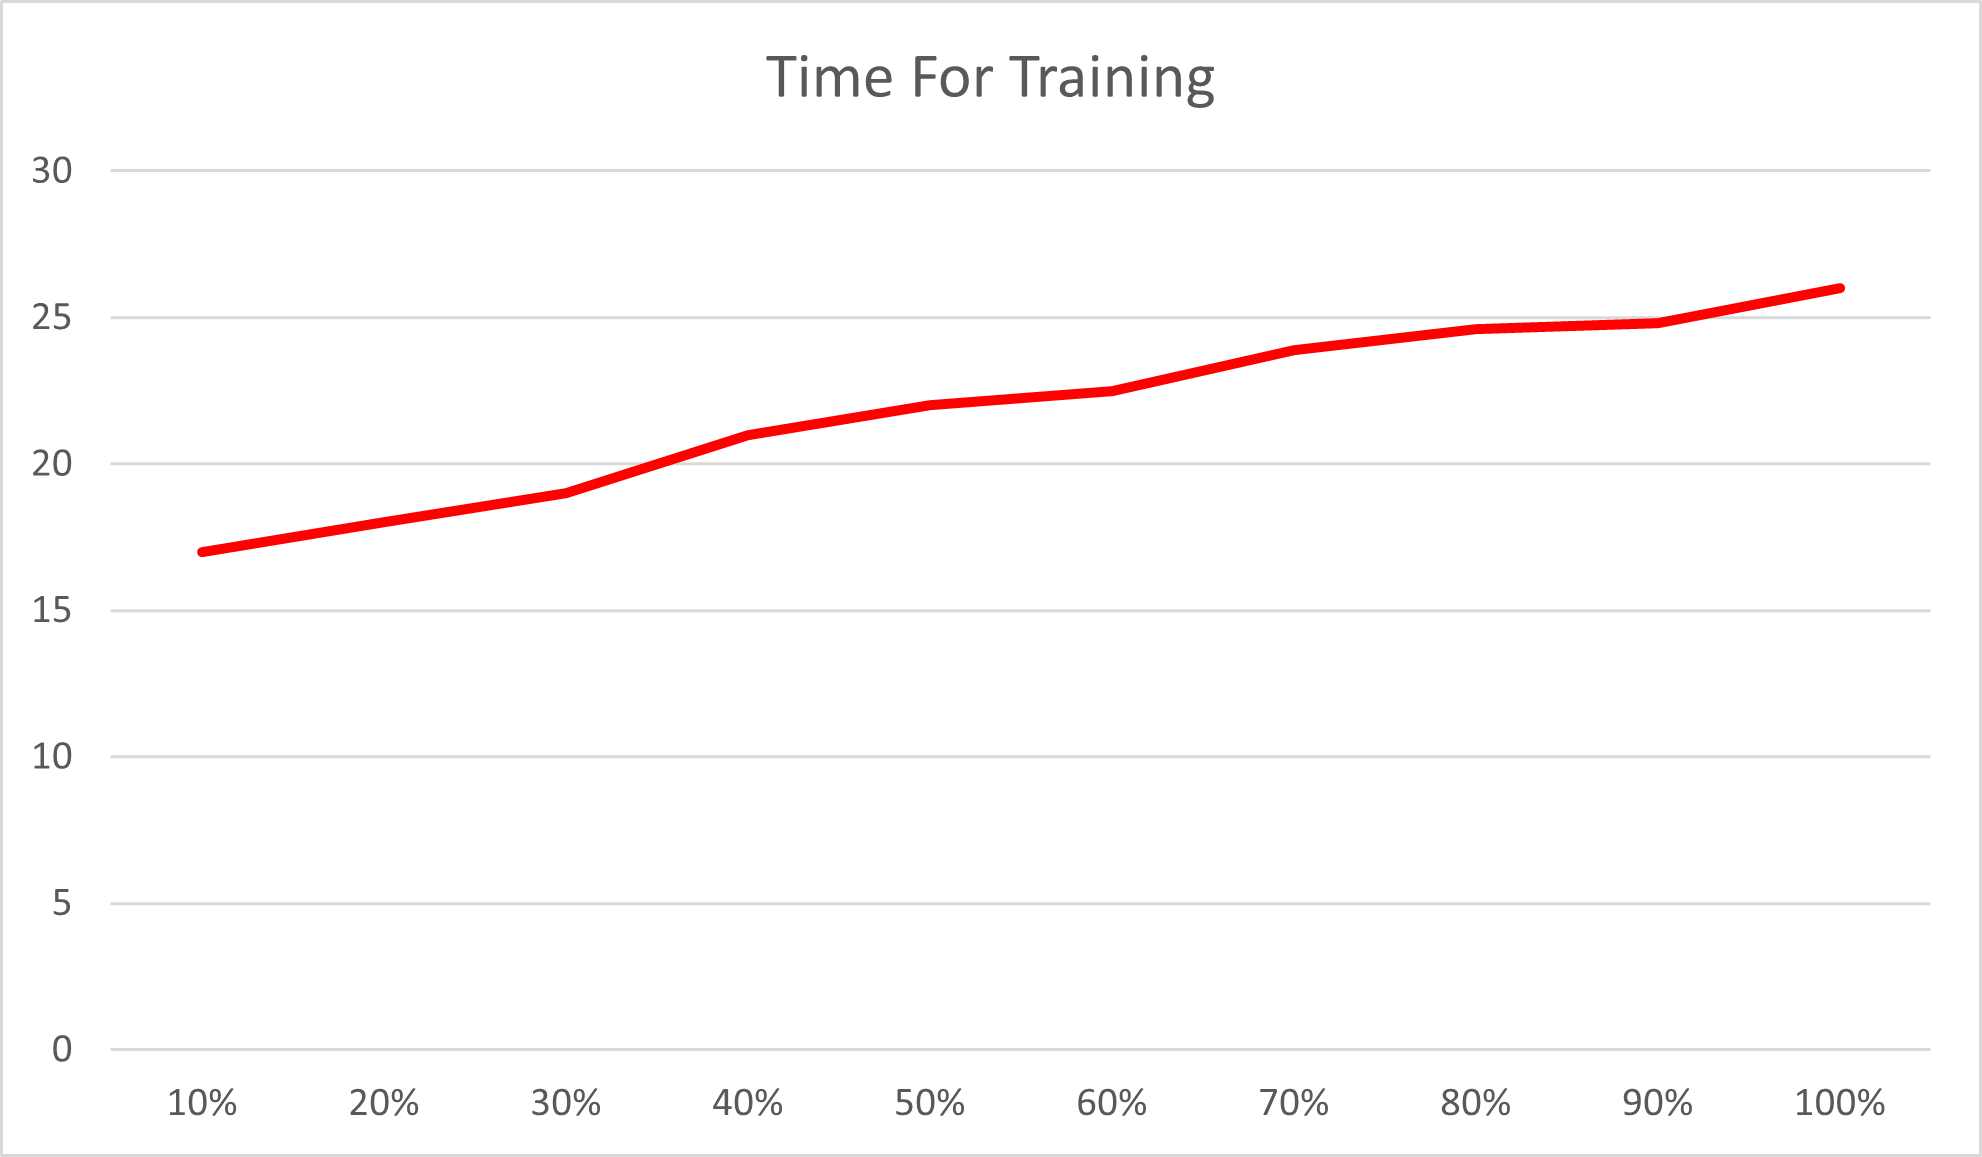
\includegraphics[width=0.7\textwidth]{Time for training NB Digit.png}}
            \item 
            \caption{Naive Bayes Digits Classifier Training}
        \end{figure}

\item
\begin{figure}[h!]
            \centering
            \IfFileExists{Accuracy NB Digit.png}{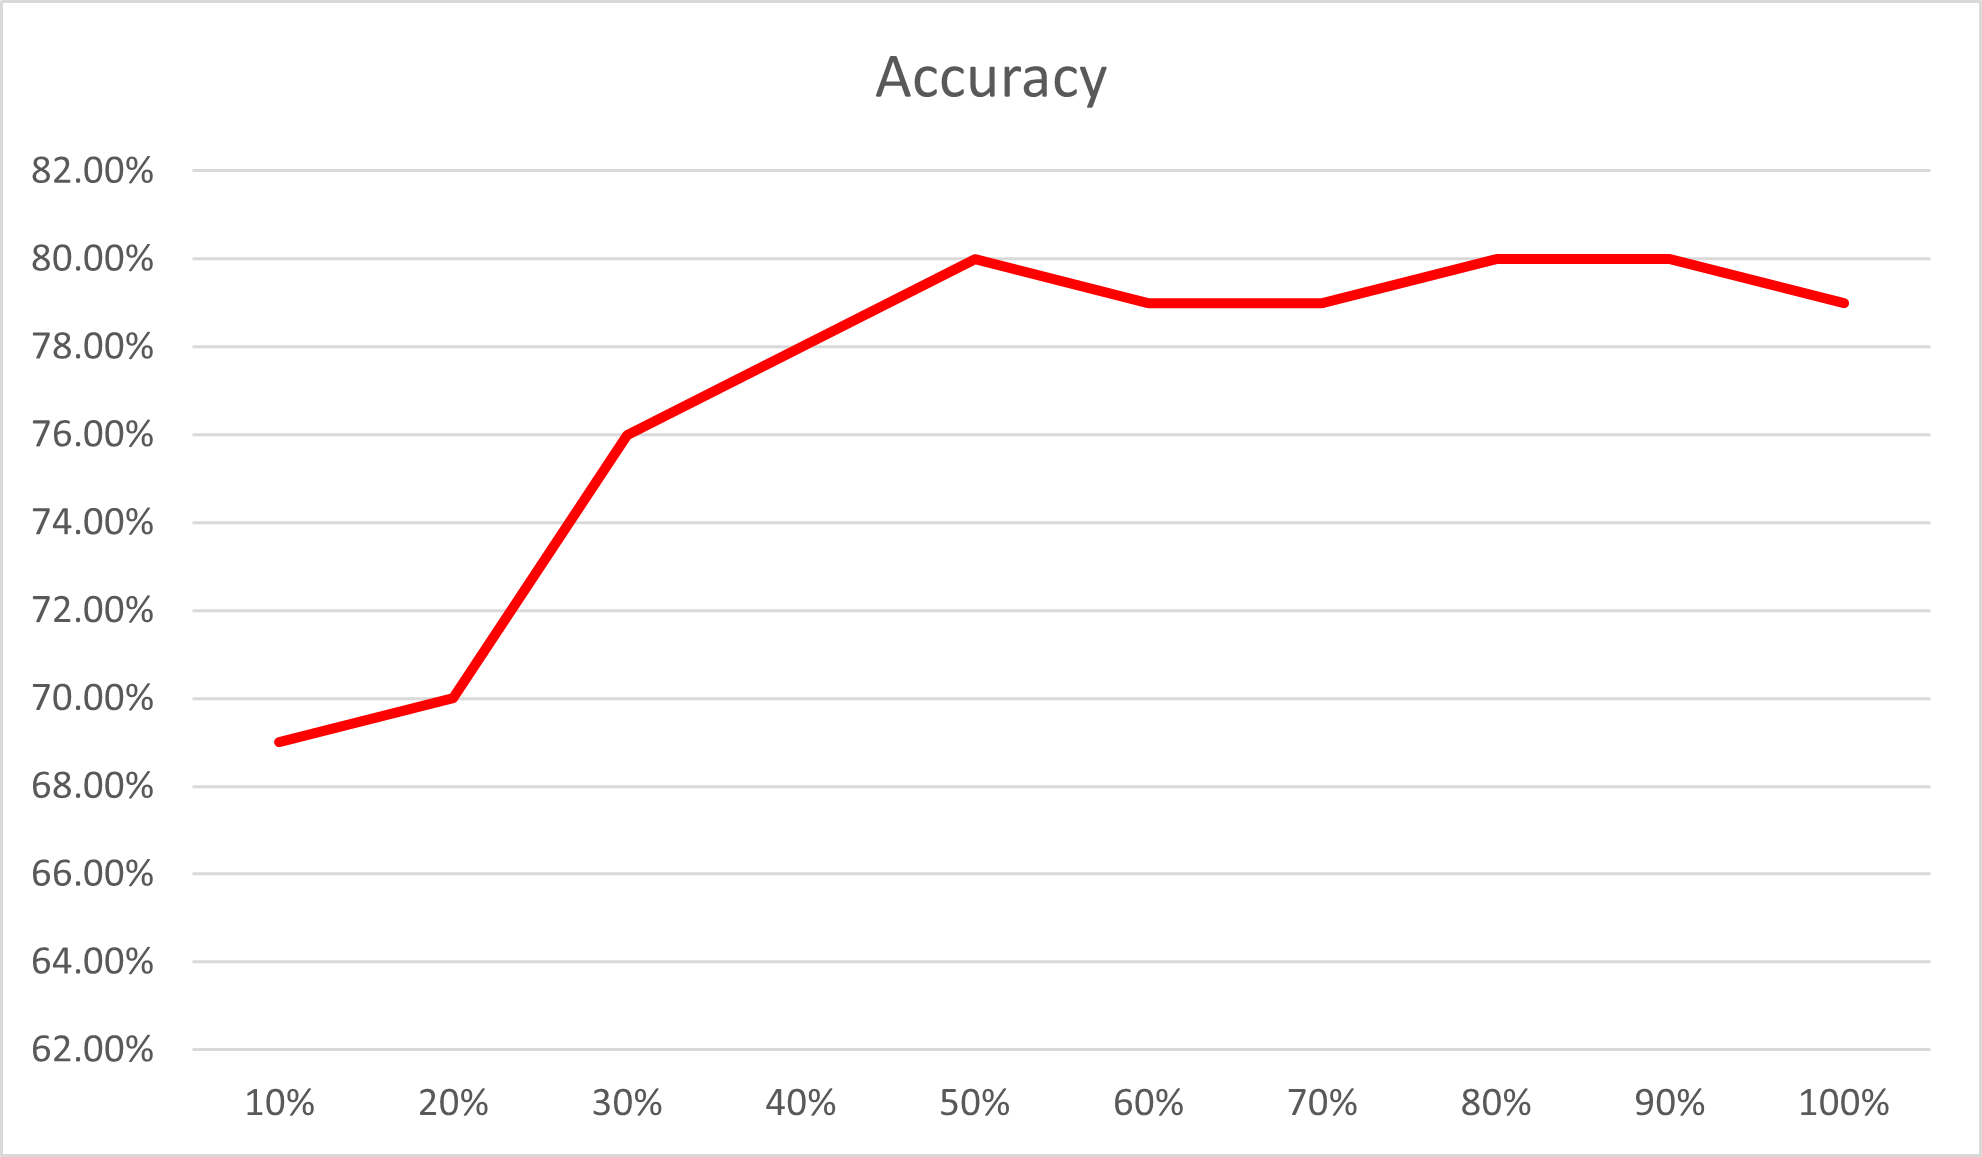
\includegraphics[width=0.7\textwidth]{Accuracy NB Digit.png}}
            \item 
            \caption{Naive Bayes Accuracy of Digits Classification}
        \end{figure}
        
\item
\begin{figure}[h!]
            \centering
            \IfFileExists{Standard deviation NB Digit.png}{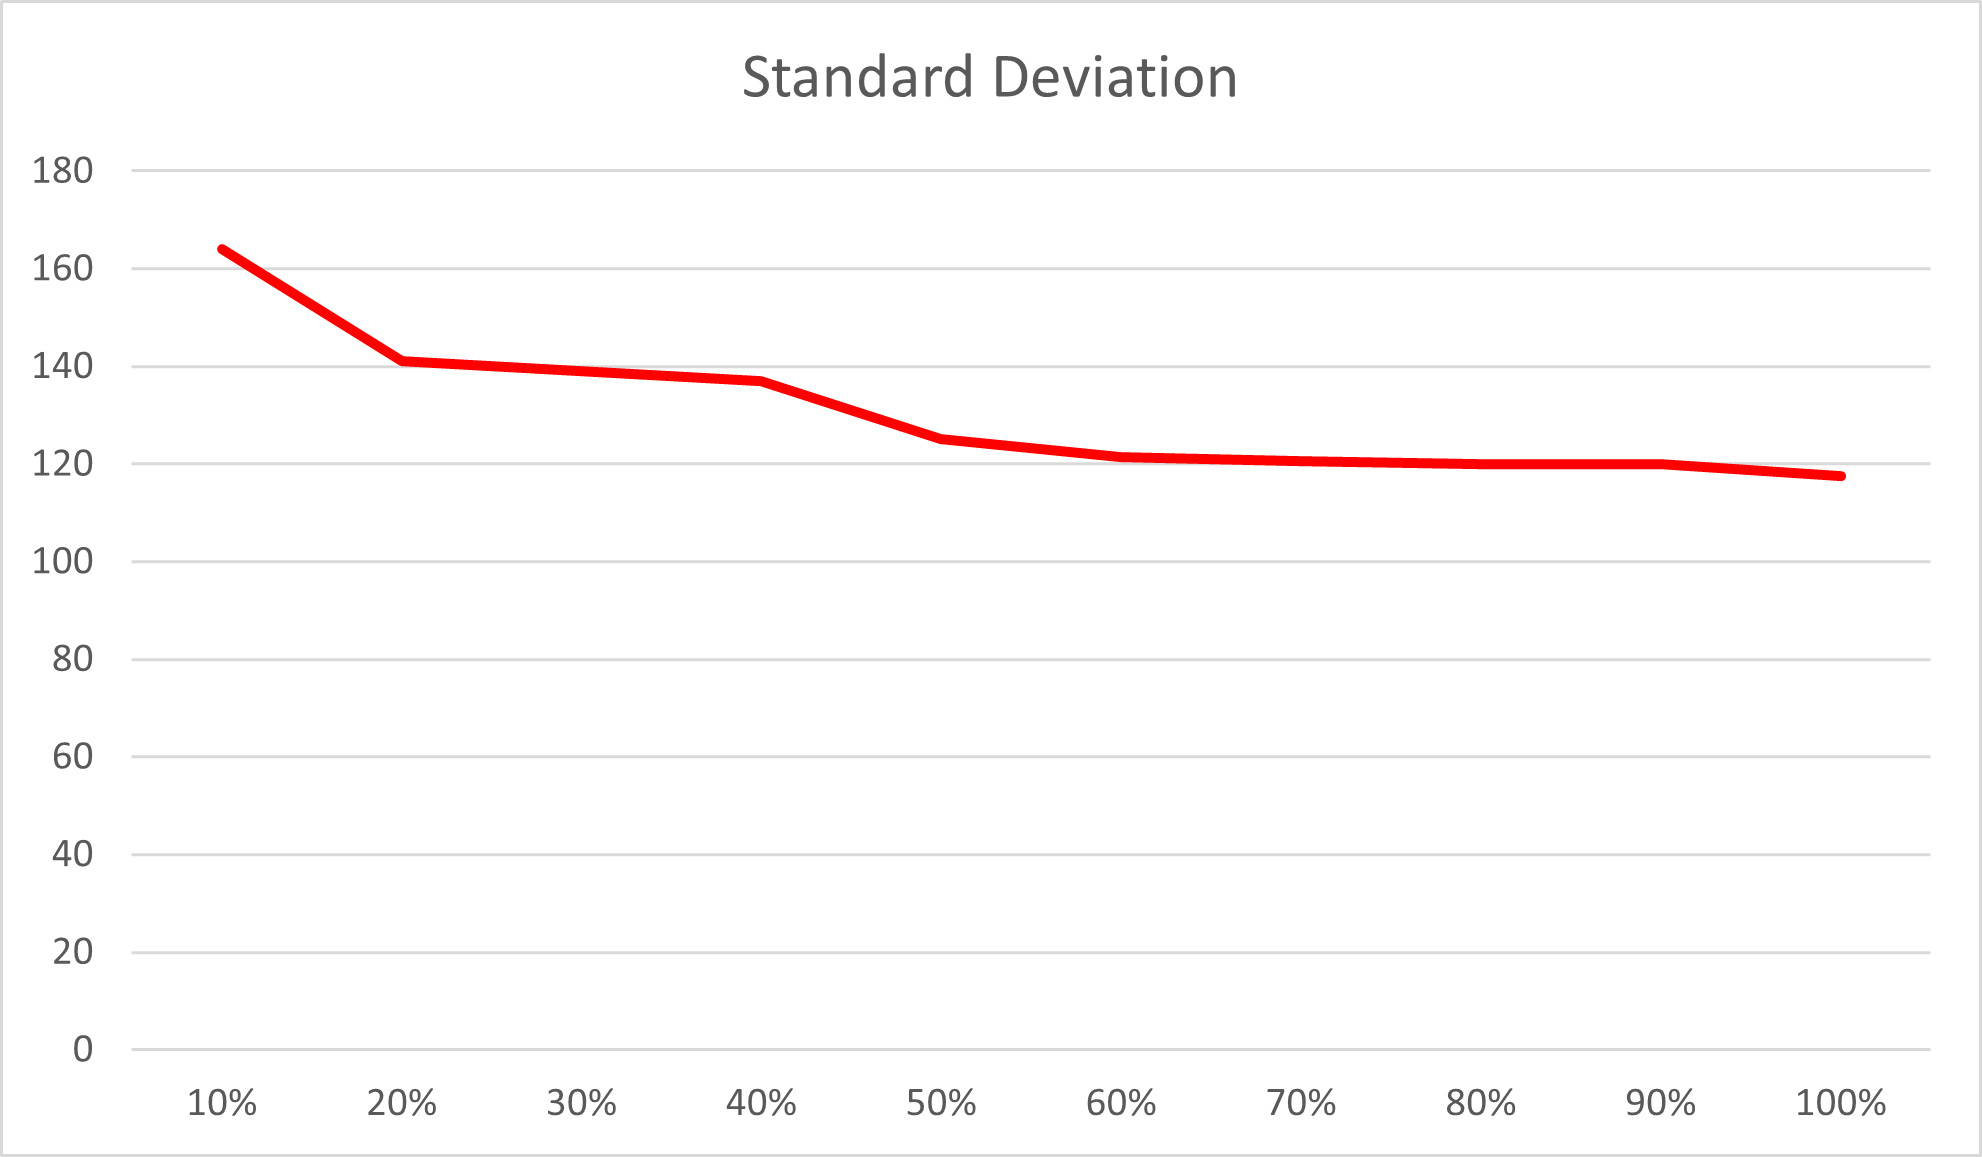
\includegraphics[width=0.7\textwidth]{Standard deviation NB Digit.png}}
            \item 
            \caption{Naive Bayes Standard Deviation of Digits Classification}
        \end{figure}

\begin{newpage}
\end{newpage}

\item \textbf{Naive Bayes Faces}
\item For Faces classifying we tested our program in increments of 10\% (10\%, 20\%, 30\%,..., 90\%, 100\%), of the total training data size. Standard deviation and accuracy was found on 100\% of the total testing data size. The following graphs were created to show the time for training (in seconds), accuracy (in percentage), and standard deviation of the data sizes tested. 

\item \textbf{Naive Bayes Faces Classification:}

\begin{figure}[h!]
            \centering
            \IfFileExists{Time for training NB Faces.png}{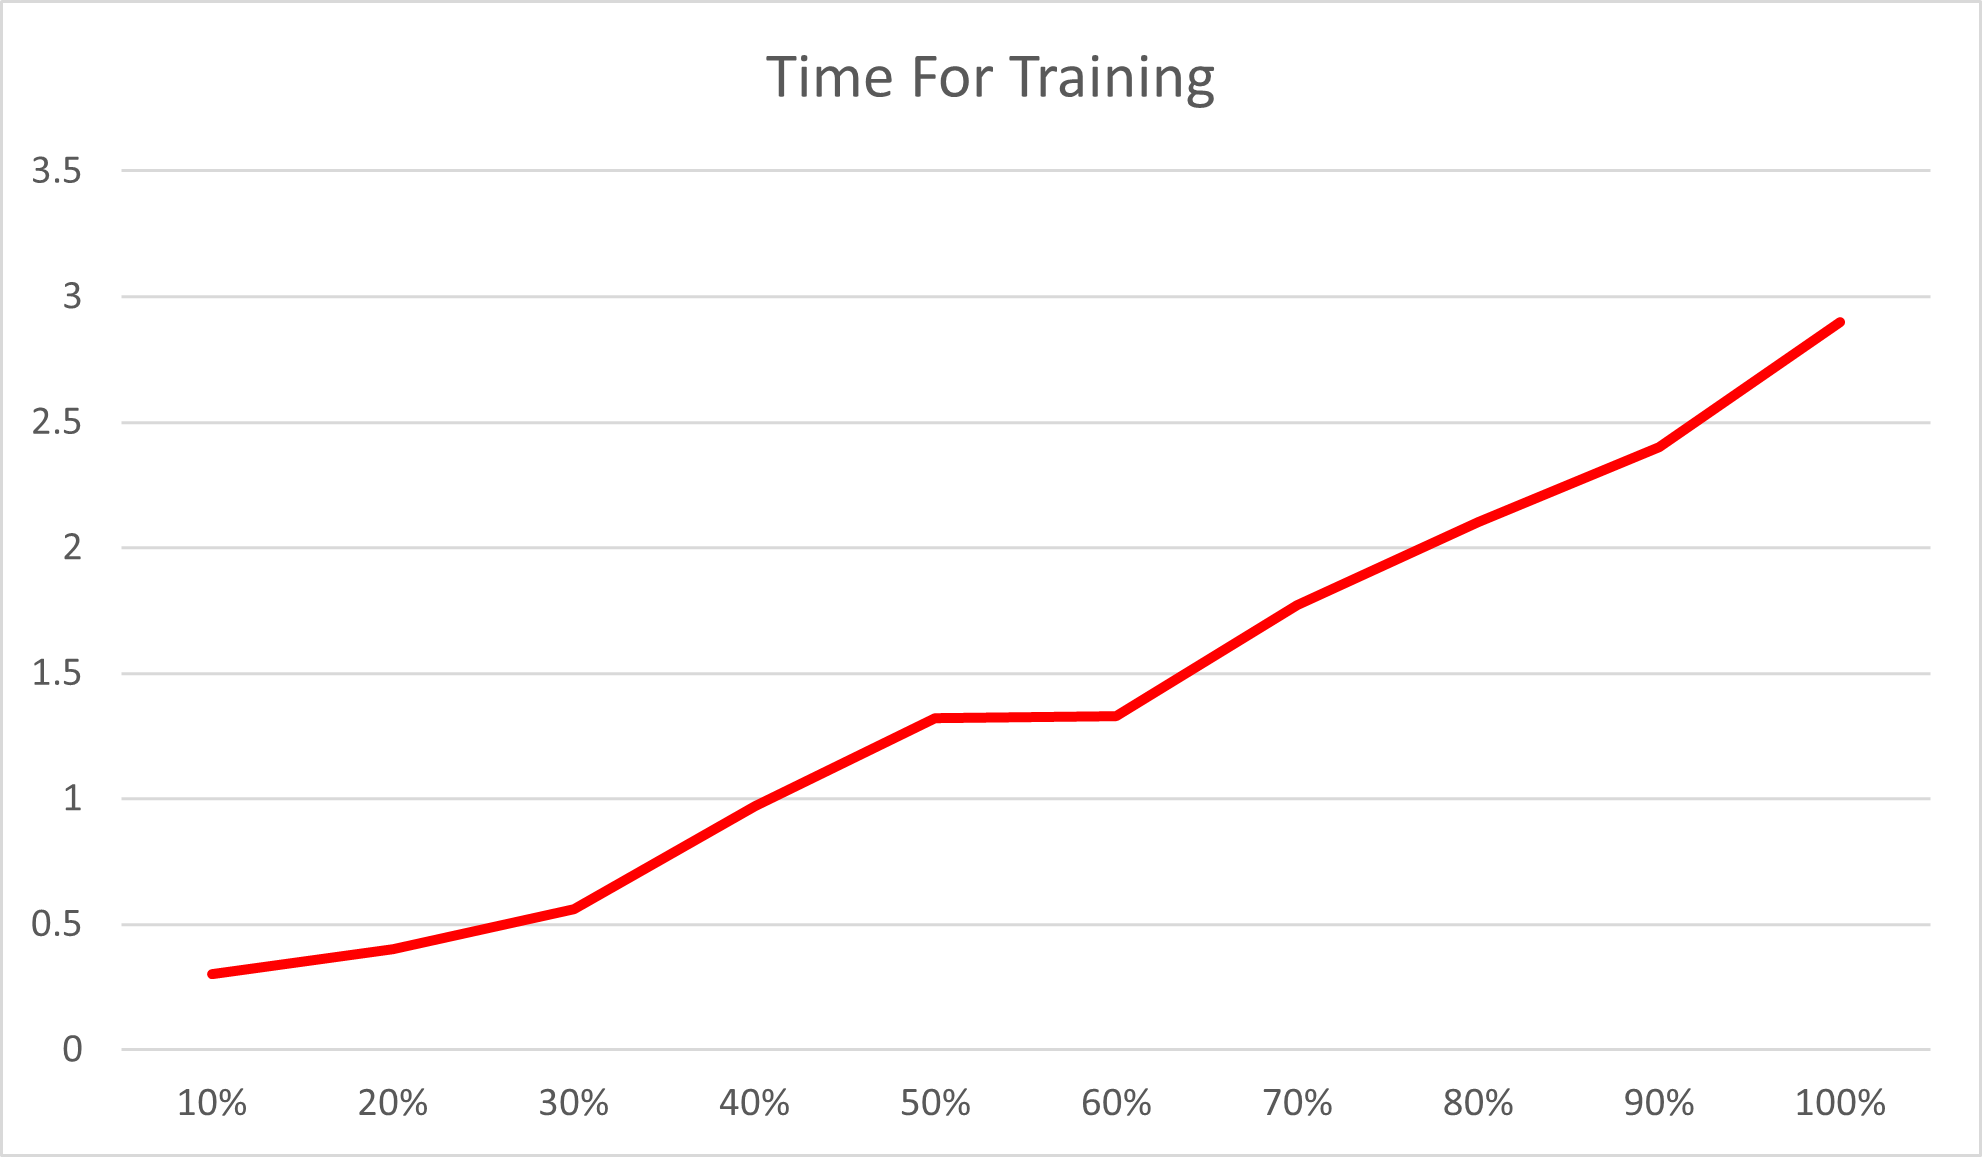
\includegraphics[width=0.7\textwidth]{Time for training NB Faces.png}}
            \item 
            \caption{Naive Bayes Faces Classifier Training}
        \end{figure}

\item
\begin{figure}[h!]
            \centering
            \IfFileExists{Accuracy NB Faces.png}{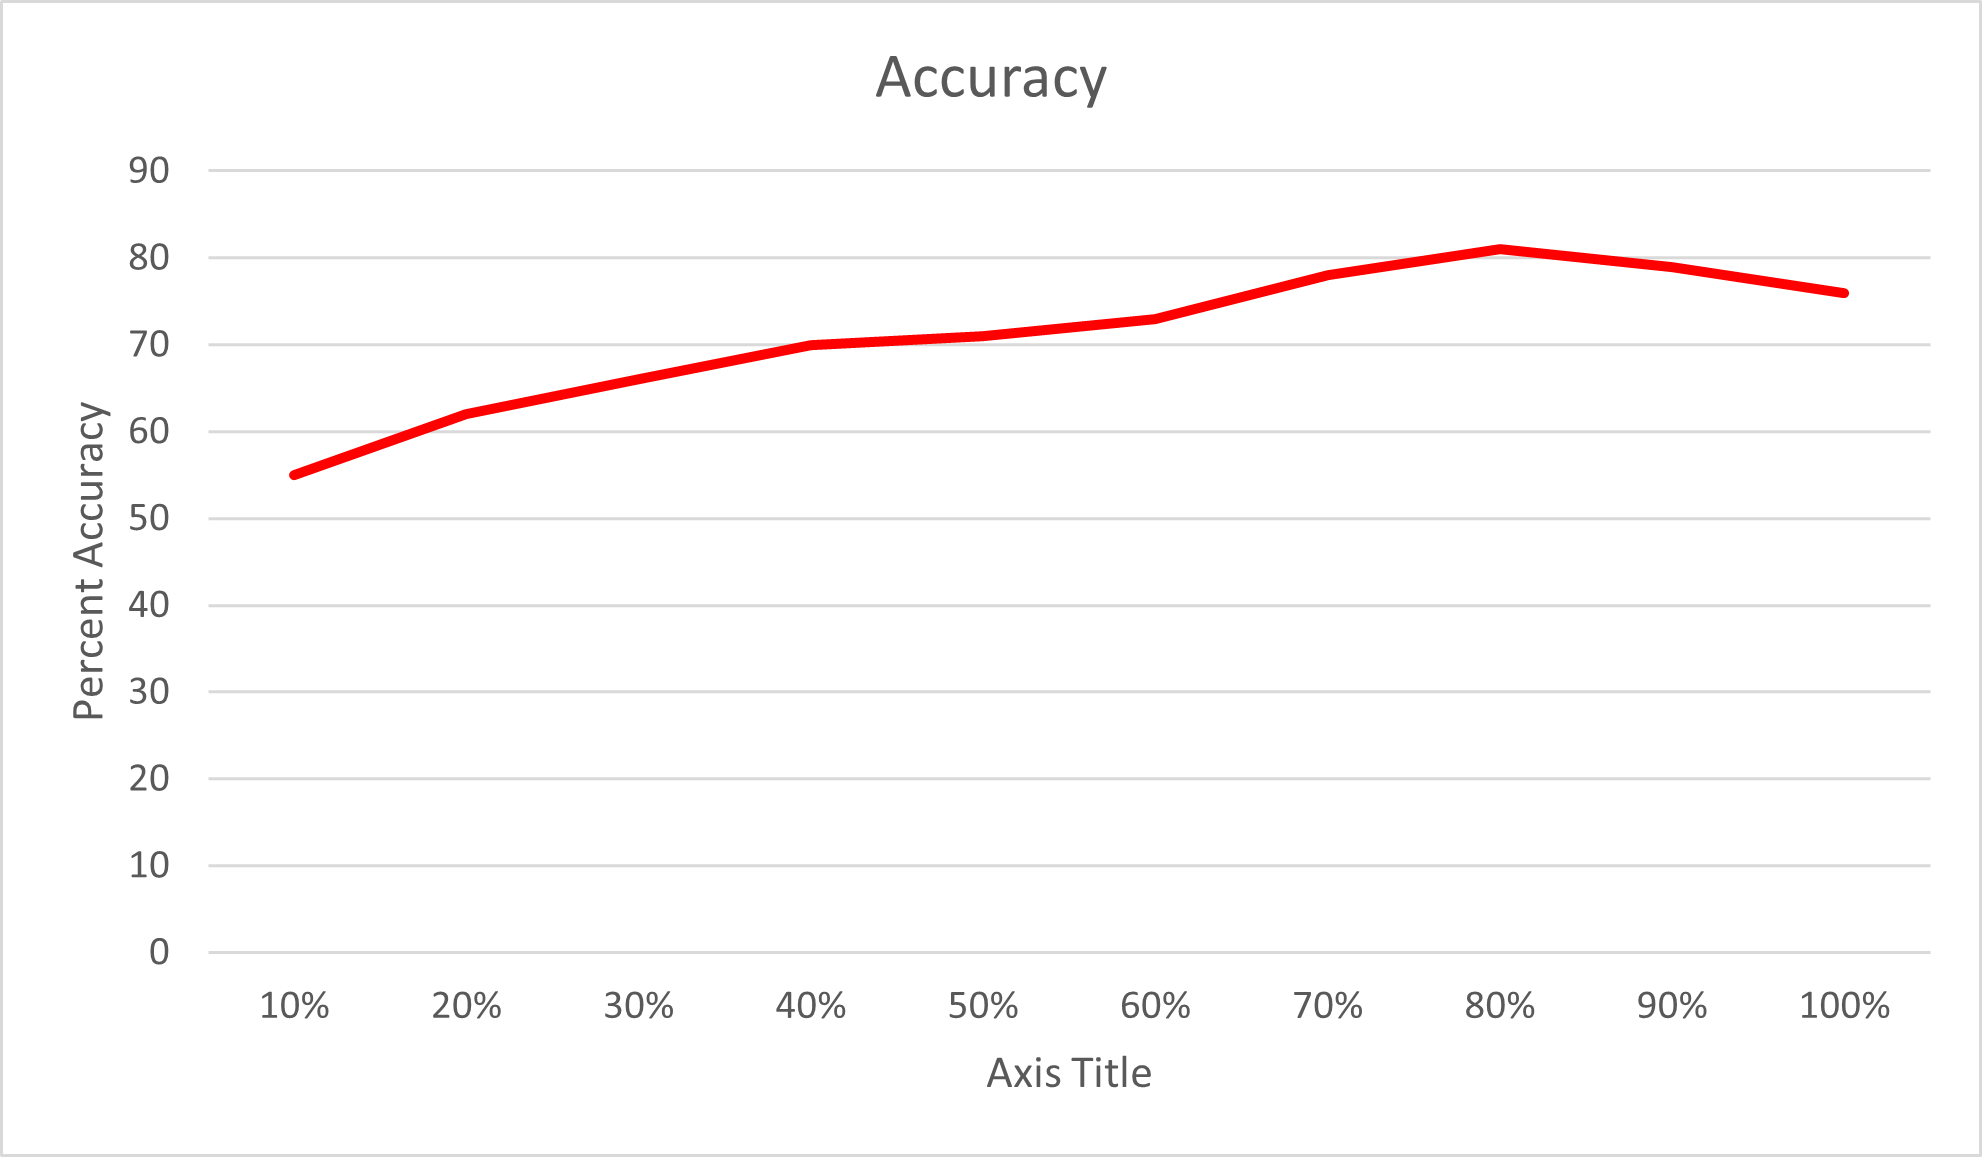
\includegraphics[width=0.7\textwidth]{Accuracy NB Faces.png}}
            \item 
            \caption{Naive Bayes Accuracy of Faces Classification}
        \end{figure}
        
\item
\begin{figure}[h!]
            \centering
            \IfFileExists{Standard deviation NB Faces.png}{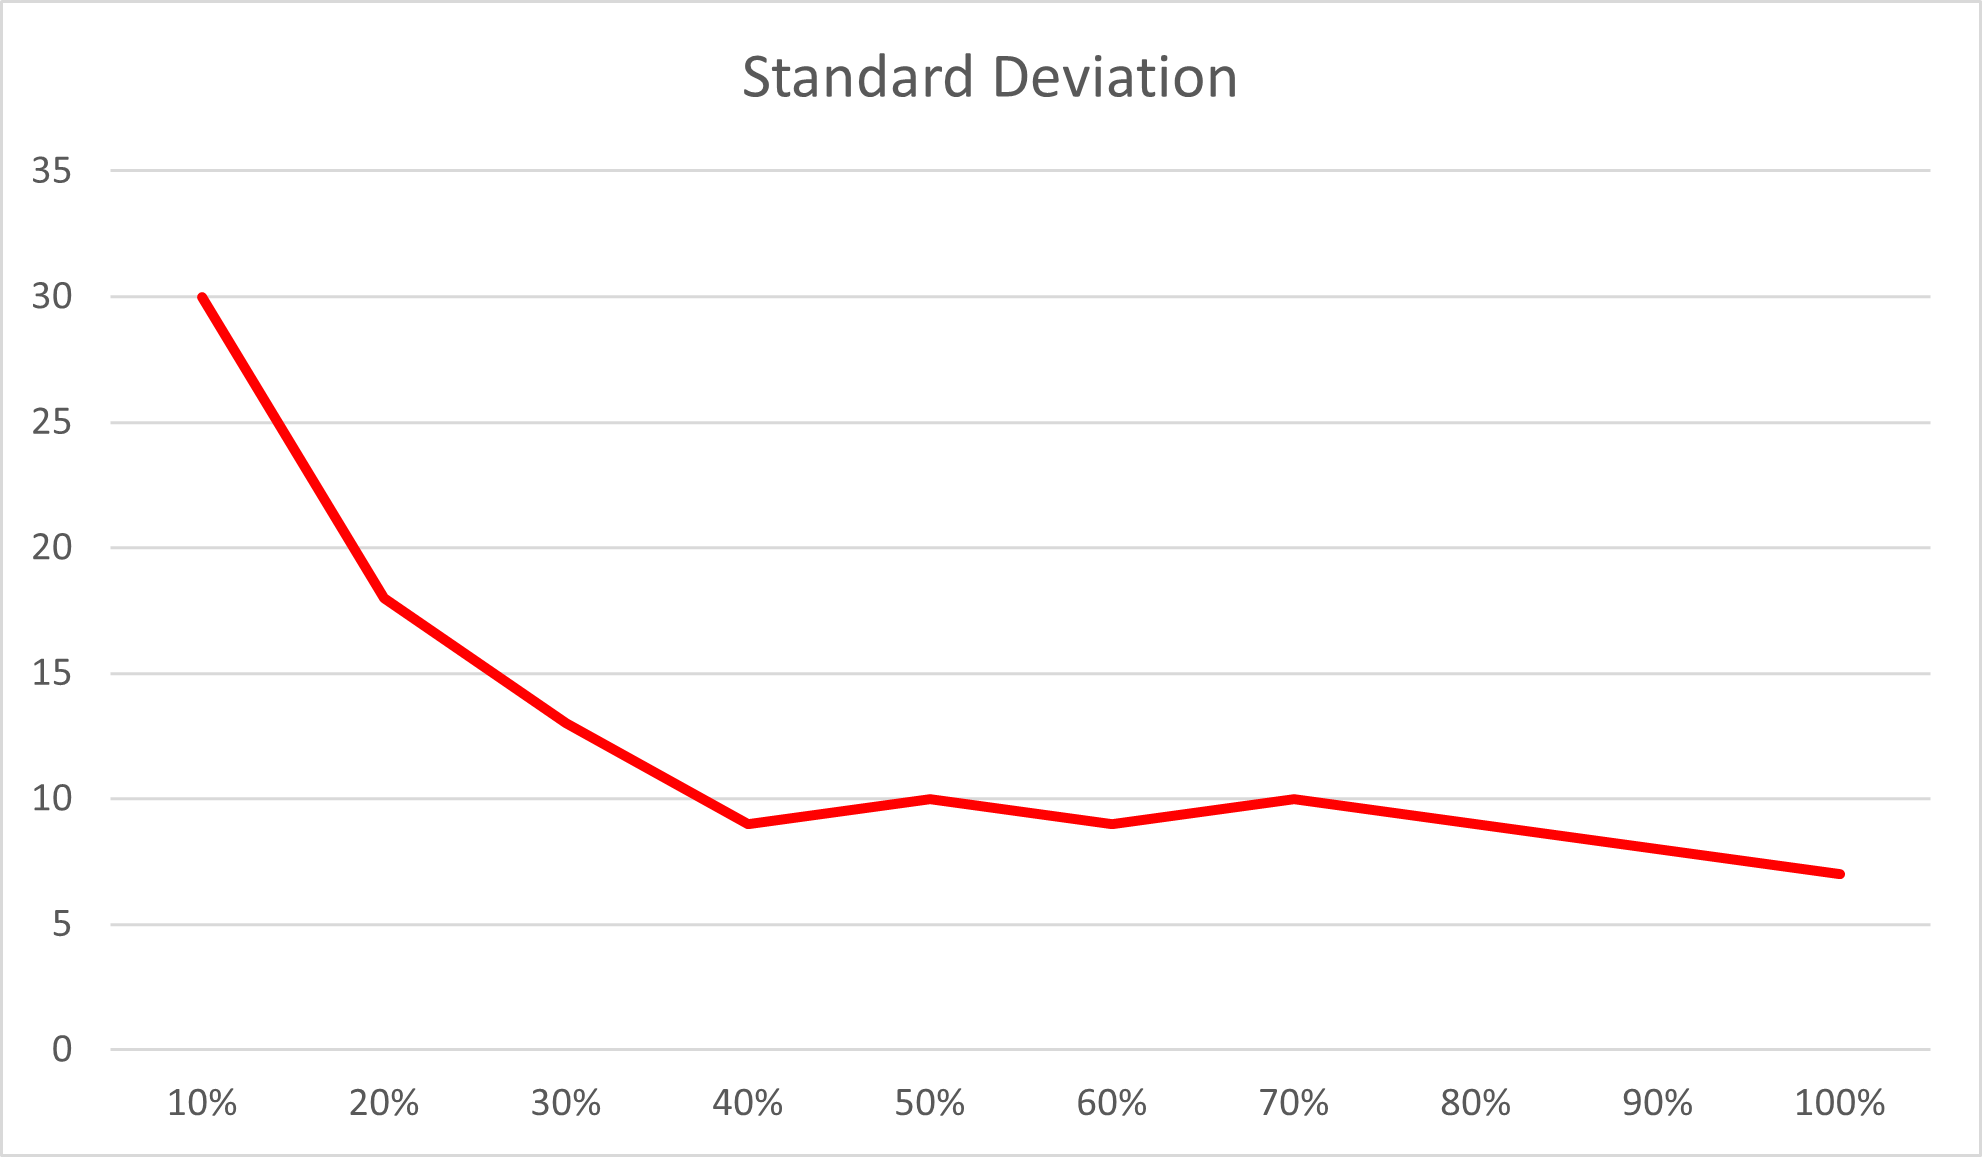
\includegraphics[width=0.7\textwidth]{Standard deviation NB Faces.png}}
            \item 
            \caption{Naive Bayes Standard Deviation of Faces Classification}
        \end{figure}

\begin{newpage}
\end{newpage}

%------------------------%
\item \textbf{Perceptron}
\item \textbf{Perceptron Digits Classification}
\item We approached this algorithm similar to how we did Naive Bayes as just a set of pixel features. For each pixel $\phi_j$ it can take either value of a white pixel as 0 or a black/grey pixel as 1. We created a dictionary,key labeled Y, containing the coordinate of the pixels as keys containing 0s and 1s. In the algorithm, we initialized all weight to 0s from the beginning then modified them.
\item To train the program, we set a max iteration number. When the number was reached the program terminated the training sequence. We kept a list of weights to features in the dictionary. The key is the legal label and the value is the list of weights. We iterated over all training data and computed a list of numbers of all legal labels using this equation:
\item $f(x_i, w) = w_0 + w_1\phi_1 + ... + w_j\phi_j$
\item We picked the label with the highest $f(x_i, w)$ as our guess. If $guess == label$, then we correctly predicted the label correctly and no change was necessary. If $guess != label$, then the weight list for the correct label was too small and the weight list for our guess was too large. This was our proceeding step:
\item for $i = 1,2,....,j : weights[label][i] += \phi_i(datum)$
\item $w_o += 1$
\item for $i = 1,2,....,j : weights[label][i] -= \phi_i(datum)$
\item $w_o -= 1$
\item This process was repeated until nothing changed in one iteration or the max iteration was reached.

\item For classification of a datum, we computed a list of numbers corresponding to all legal labels using the same equation as before:
\item $f(x_i, w) = w_0 + w_1\phi_1 + ... + w_j\phi_j$
\item and again picked the label with the highest $f(x_i, w)$ as our guess.

\item For digits classifying, we tested our program through increments of 10\% (10\%, 20\%, 30\%,..., 90\%, 100\%) of the total training data size. Standard deviation and accuracy was found on 100\% of the total testing data size. The following graphs were created to show the time for training (in seconds), accuracy (in percentage) and standard deviation of the data sizes tested.

\item \textbf{Perceptron Digits Classification:}
\begin{figure}[h!]
            \centering
            \IfFileExists{Time for training P Digit.png}{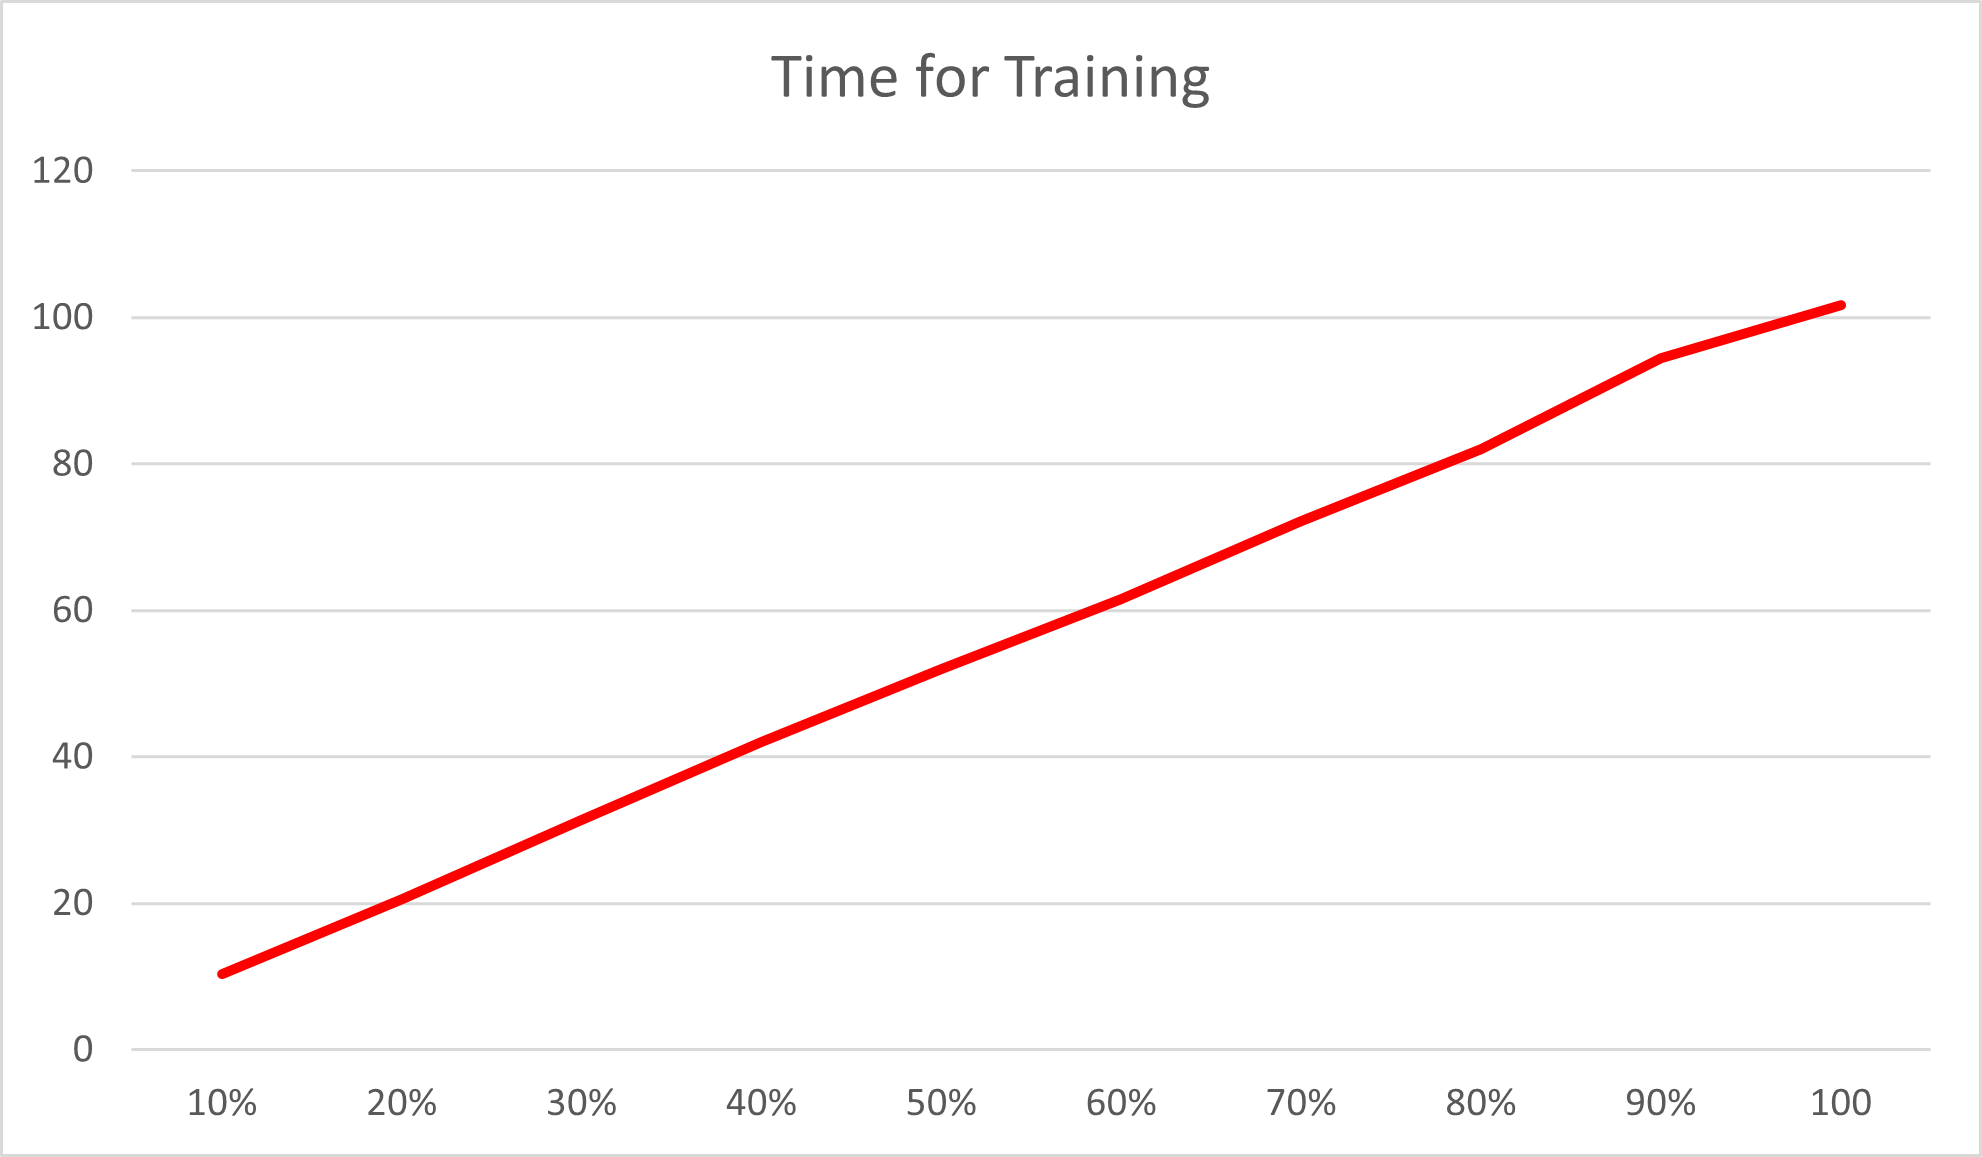
\includegraphics[width=0.7\textwidth]{Time for training P Digit.png}}
            \item 
            \caption{Perceptron Digits Classifier Training Time}
        \end{figure}
\item
\begin{figure}[h!]
            \centering
            \IfFileExists{Accuracy P Digit.png}{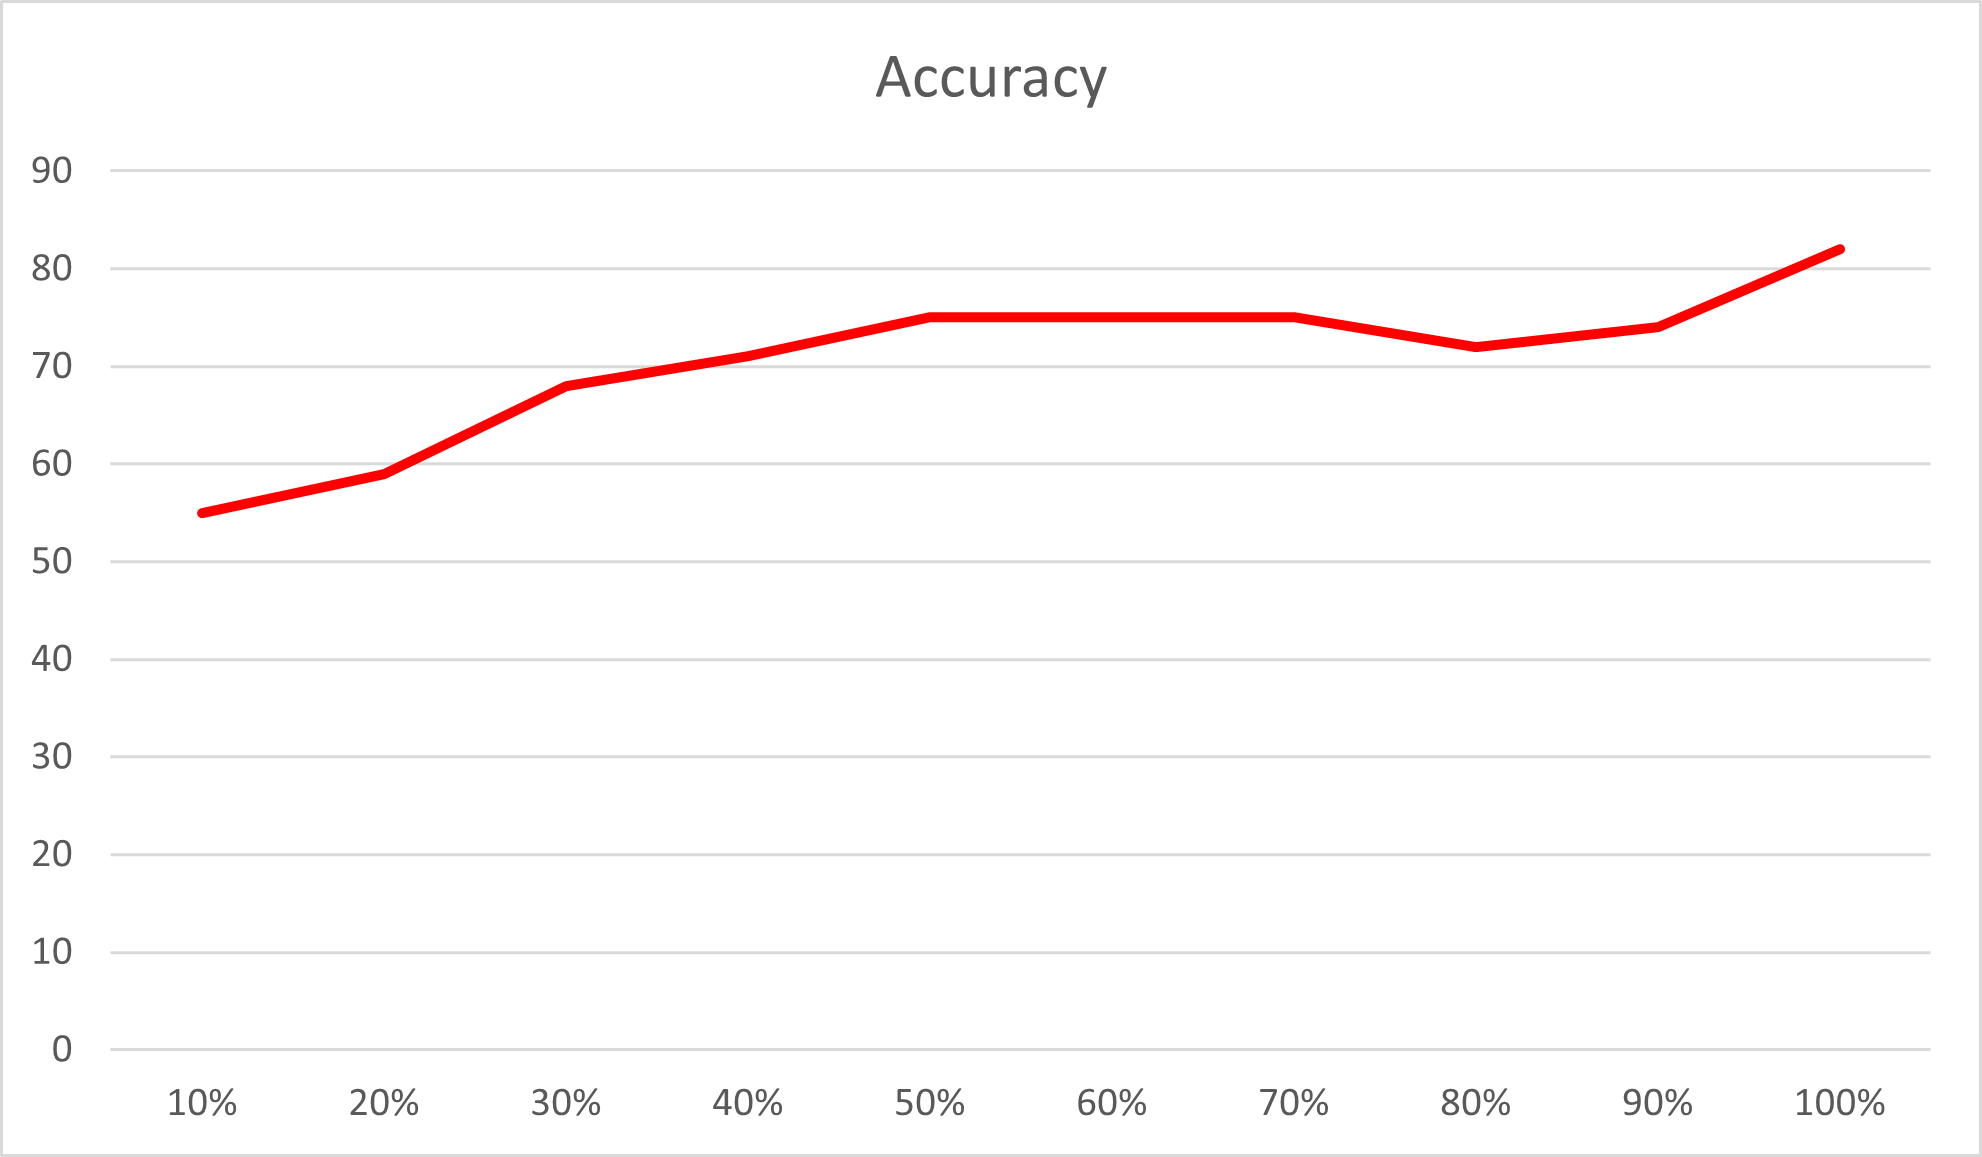
\includegraphics[width=0.7\textwidth]{Accuracy P Digit.png}}
            \item 
            \caption{Perceptron Accuracy of Digits Classification}
        \end{figure}
        
\item
\begin{figure}[h!]
            \centering
            \IfFileExists{Standard deviation P Digit.png}{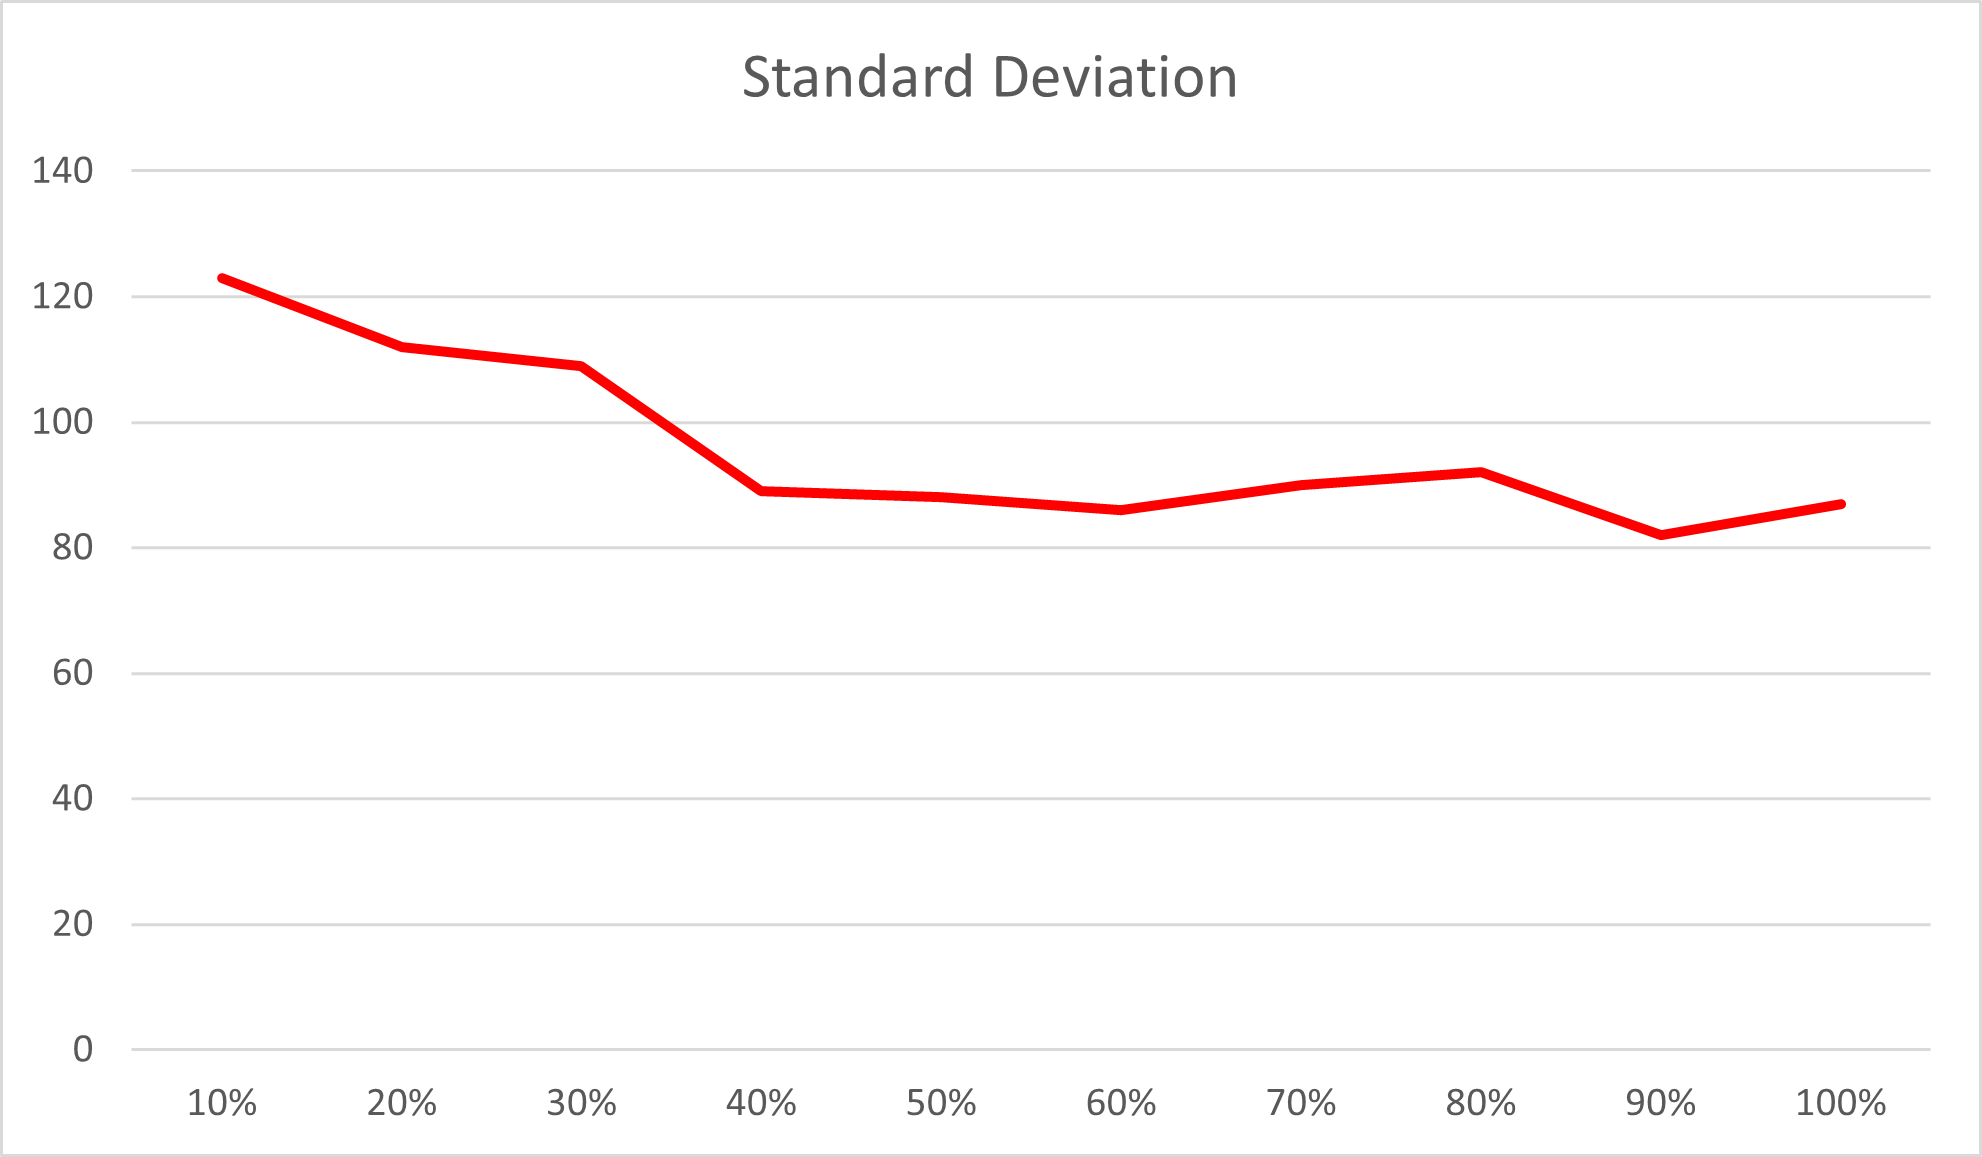
\includegraphics[width=0.7\textwidth]{Standard deviation P Digit.png}}
            \item 
            \caption{Percepton Standard Deviation of Digits Classification}
        \end{figure}

\begin{newpage}
\end{newpage}

\item \textbf{Perceptron Faces}
\item For Faces classifying we tested our program in increments of 10\% (10\%, 20\%, 30\%,..., 90\%, 100\%), of the total training data size. Standard deviation and accuracy was found on 100\% of the total testing data size. The following graphs were created to show the time for training (in seconds), accuracy (in percentage) and standard deviation of the data sizes tested. 

\begin{newpage}
\end{newpage}
\item \textbf{Perceptron Faces Classification:}

\begin{figure}[h!]
            \centering
            \IfFileExists{Time for training P Faces.png}{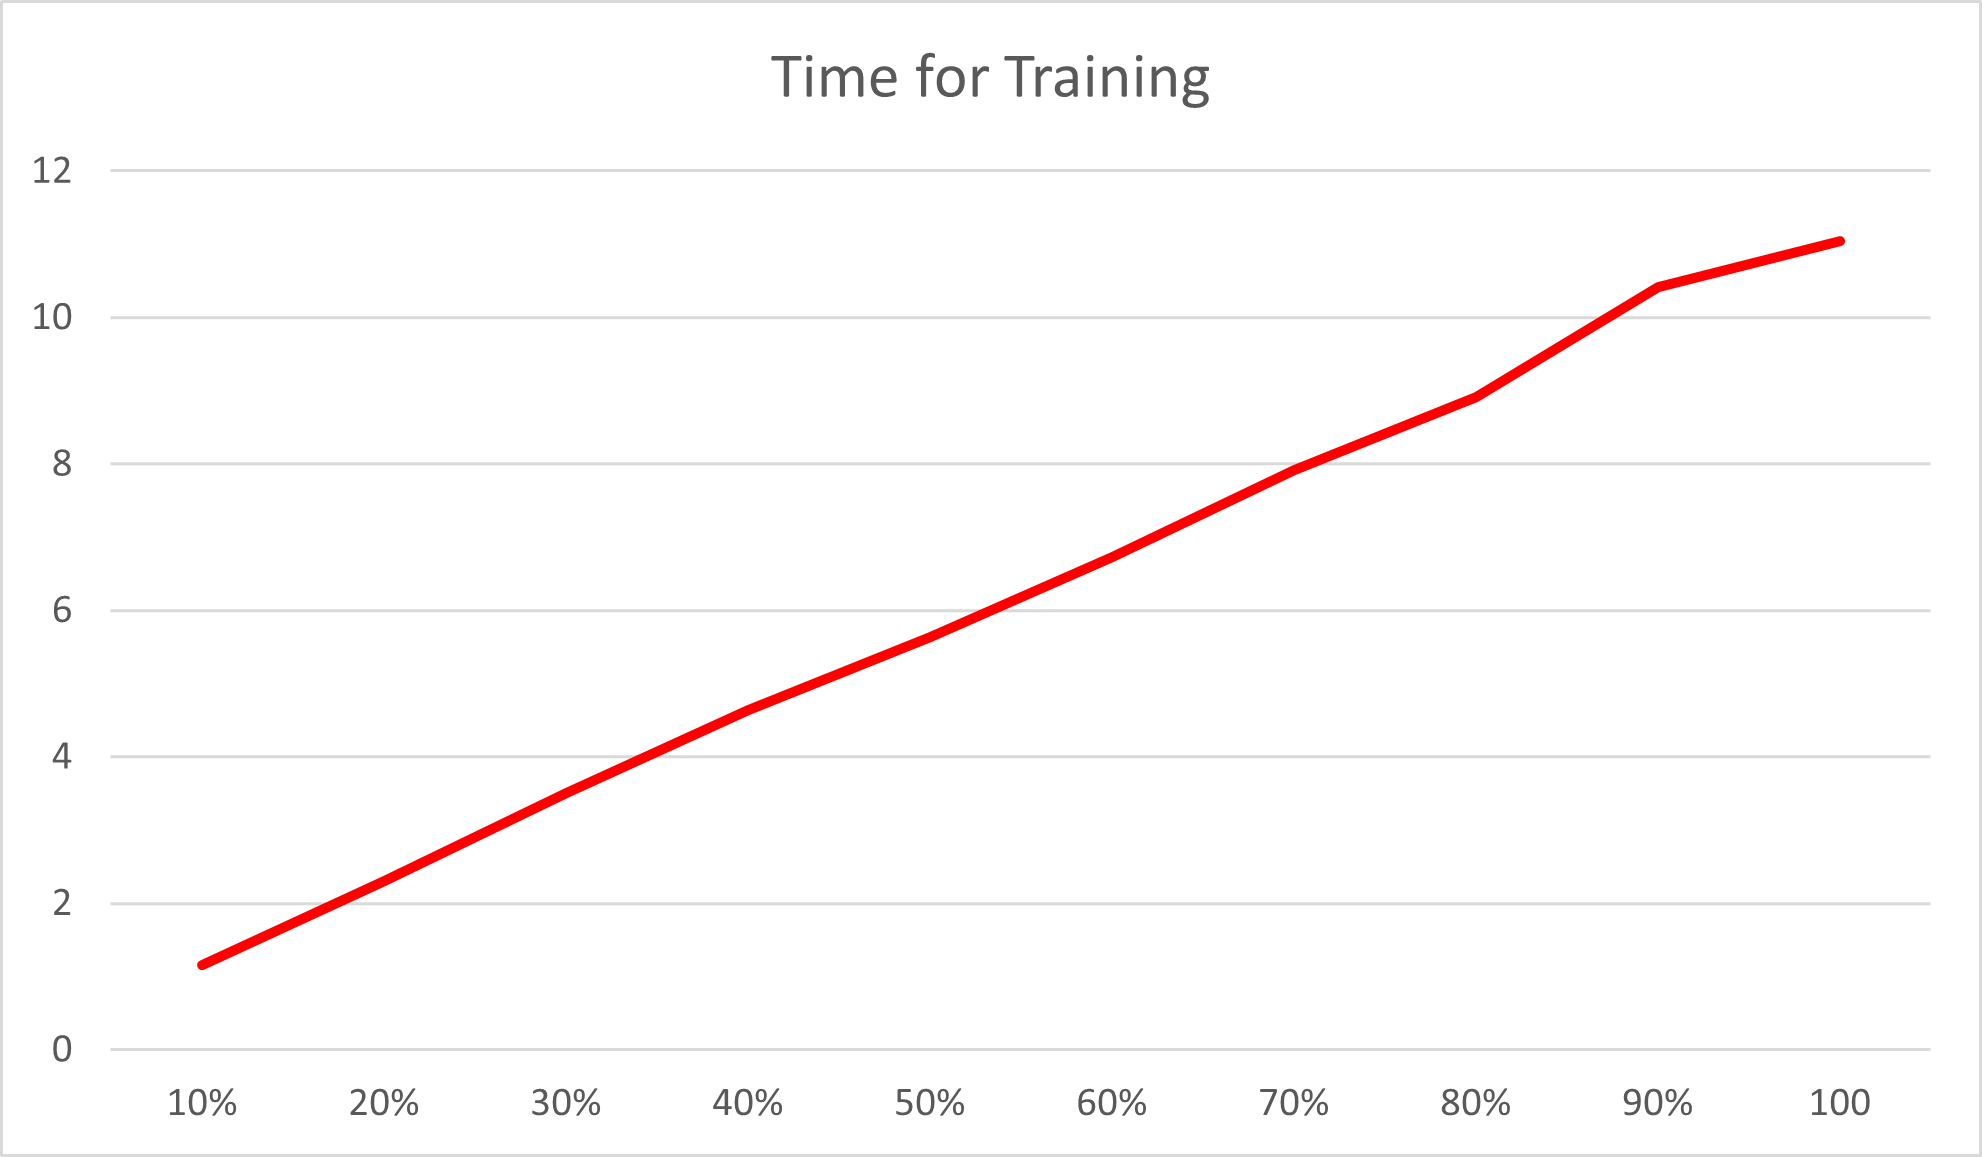
\includegraphics[width=0.7\textwidth]{Time for training P Faces.png}}
            \item 
            \caption{Perceptron Faces Classifier Training}
        \end{figure}

\item
\begin{figure}[h!]
            \centering
            \IfFileExists{Accuracy P Faces.png}{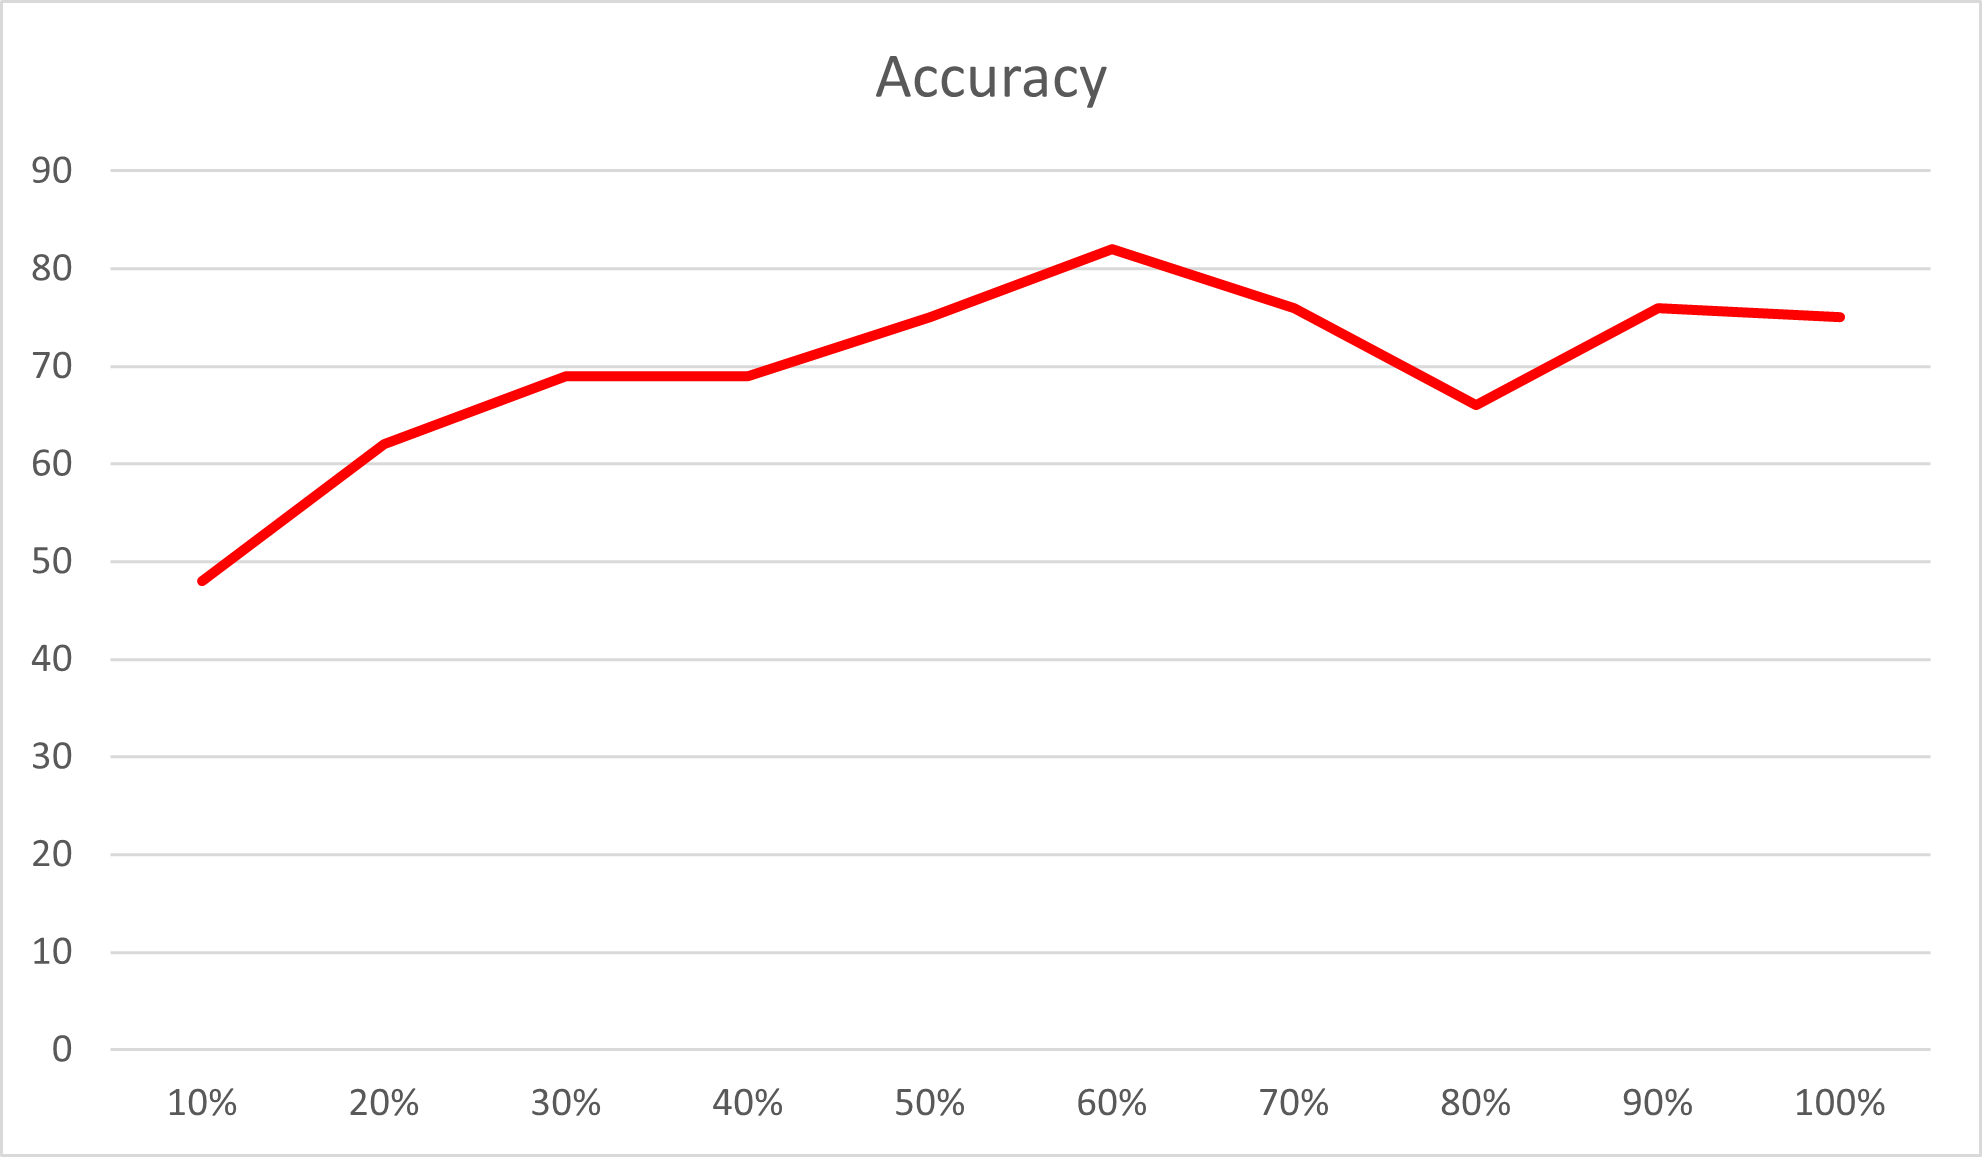
\includegraphics[width=0.7\textwidth]{Accuracy P Faces.png}}
            \item 
            \caption{Perceptron Accuracy of Faces Classification}
        \end{figure}
        
\item
\begin{figure}[h!]
            \centering
            \IfFileExists{Standard deviation P Faces.png}{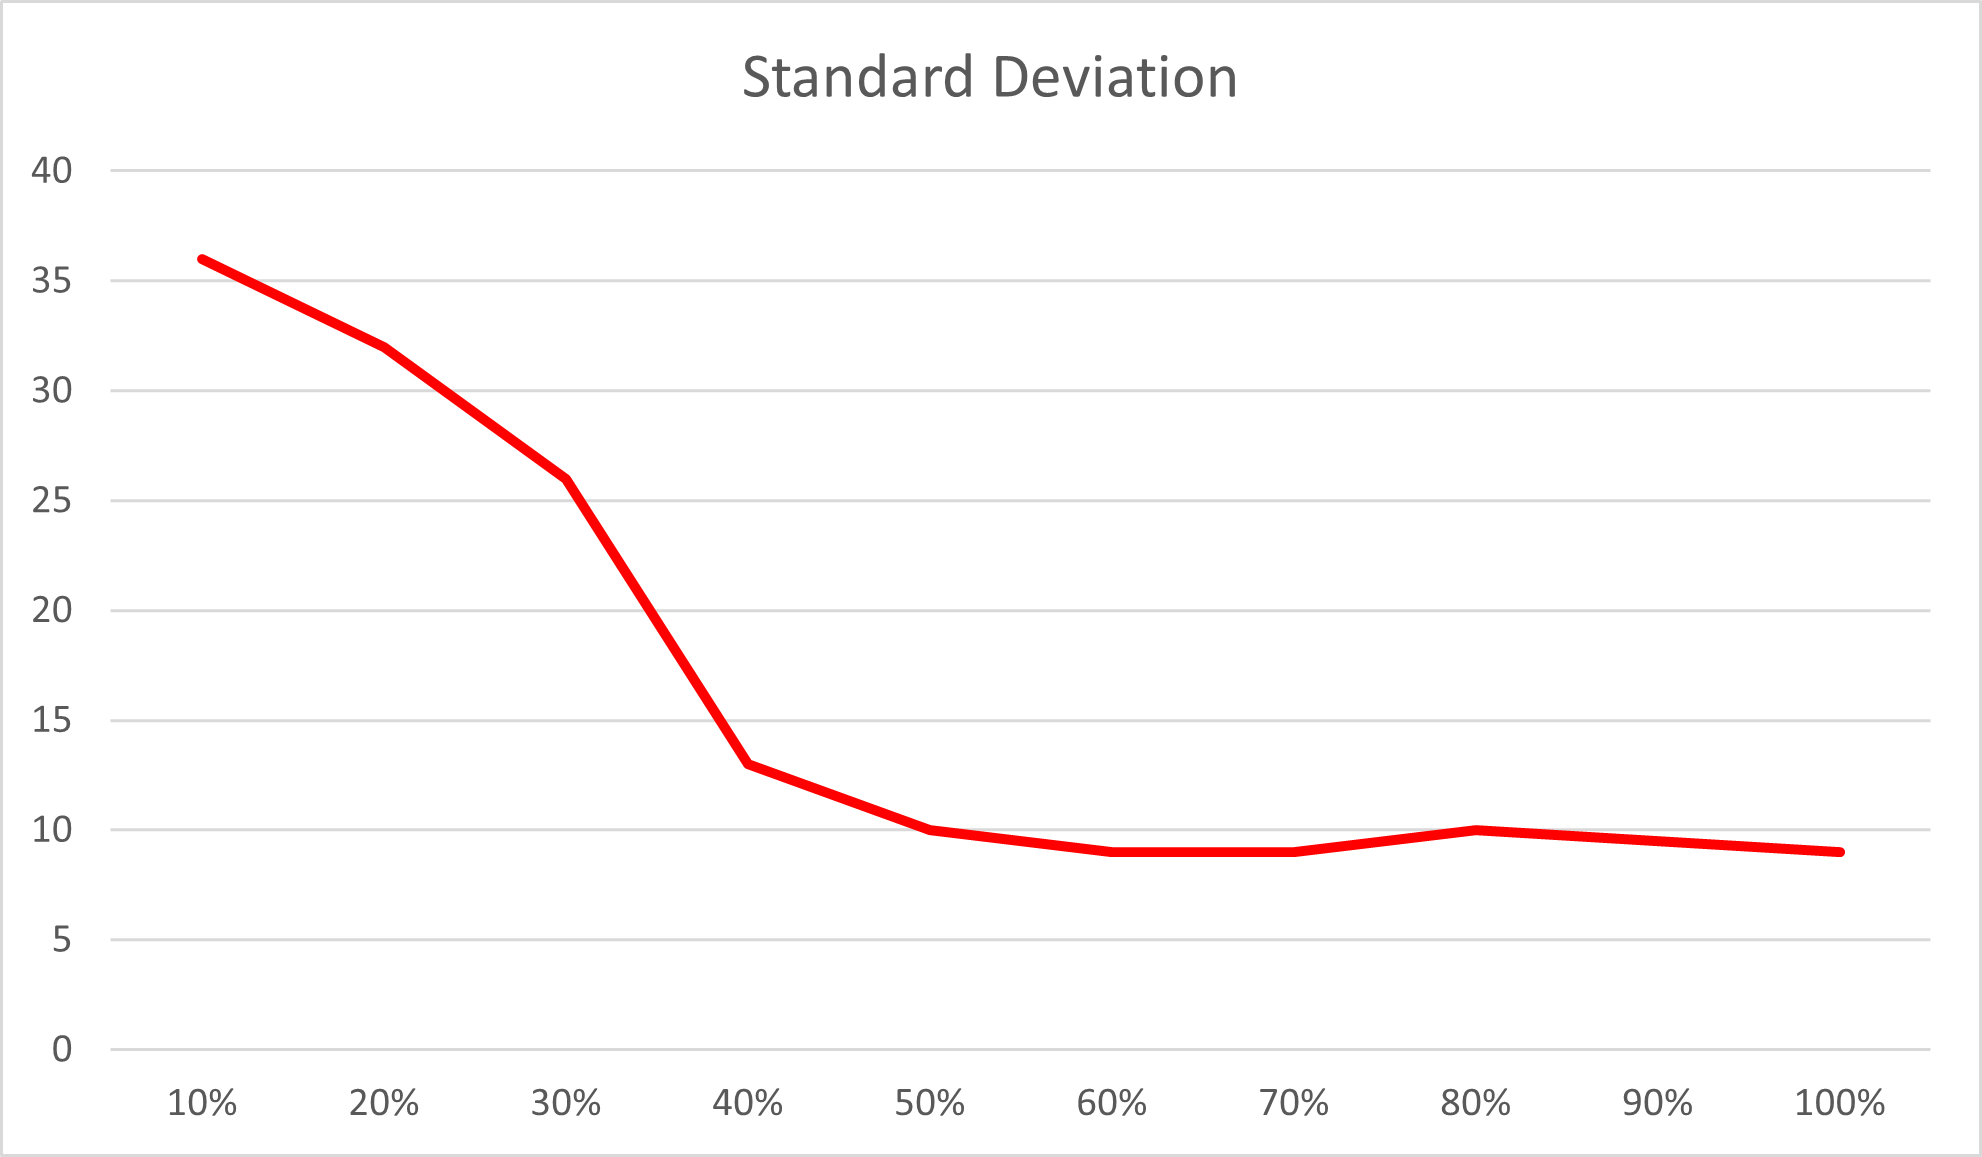
\includegraphics[width=0.7\textwidth]{Standard deviation P Faces.png}}
            \item 
            \caption{Perceptron Standard Deviation of Faces Classification}
        \end{figure}

\begin{newpage}
\end{newpage}

%------------------------%


\item \textbf{K-Nearest Neighbor}

\item We approached this algorithm by taking a sample, calculating its distance to all training samples, then classifying to the appropriate label the majority of $K$ closest samples are. We implemented KNN for its use of cosine distance. Cosine is the angle between length vectors $n$ in $n$-dimensional space and we used $m$ and $n$ as our distance vector variables. The following equation was used to determine the distance:
\item $dist(m, n) = 1 - \cos{(\theta)}$
\item $dist(m, n) = 1 - \frac{m*n}{\|m\|n\|}$

\item KNN uses a geometric series to determine the distance of the function. This distance is the length of the line segment connecting two points and was calculated with the following equation:
\item $dist(m, n) = \sqrt{\sum_{i=1}^{z}(m_i - n_i)^2}$

\item For digits classifying, we tested our program through increments of 10\% (10\%, 20\%, 30\%,..., 90\%, 100\%) of the total training data size. Standard deviation and accuracy was found on 100\% of the total testing data size. The following graphs were created to show the time for training (in seconds), accuracy (in percentage), and standard deviation of the data sizes tested. 

\begin{newpage}
\end{newpage}

\item \textbf{K Nearest Neighbor Digits Classification:}
\begin{figure}[h!]
            \centering
            \IfFileExists{Time for training KNN Digit.png}{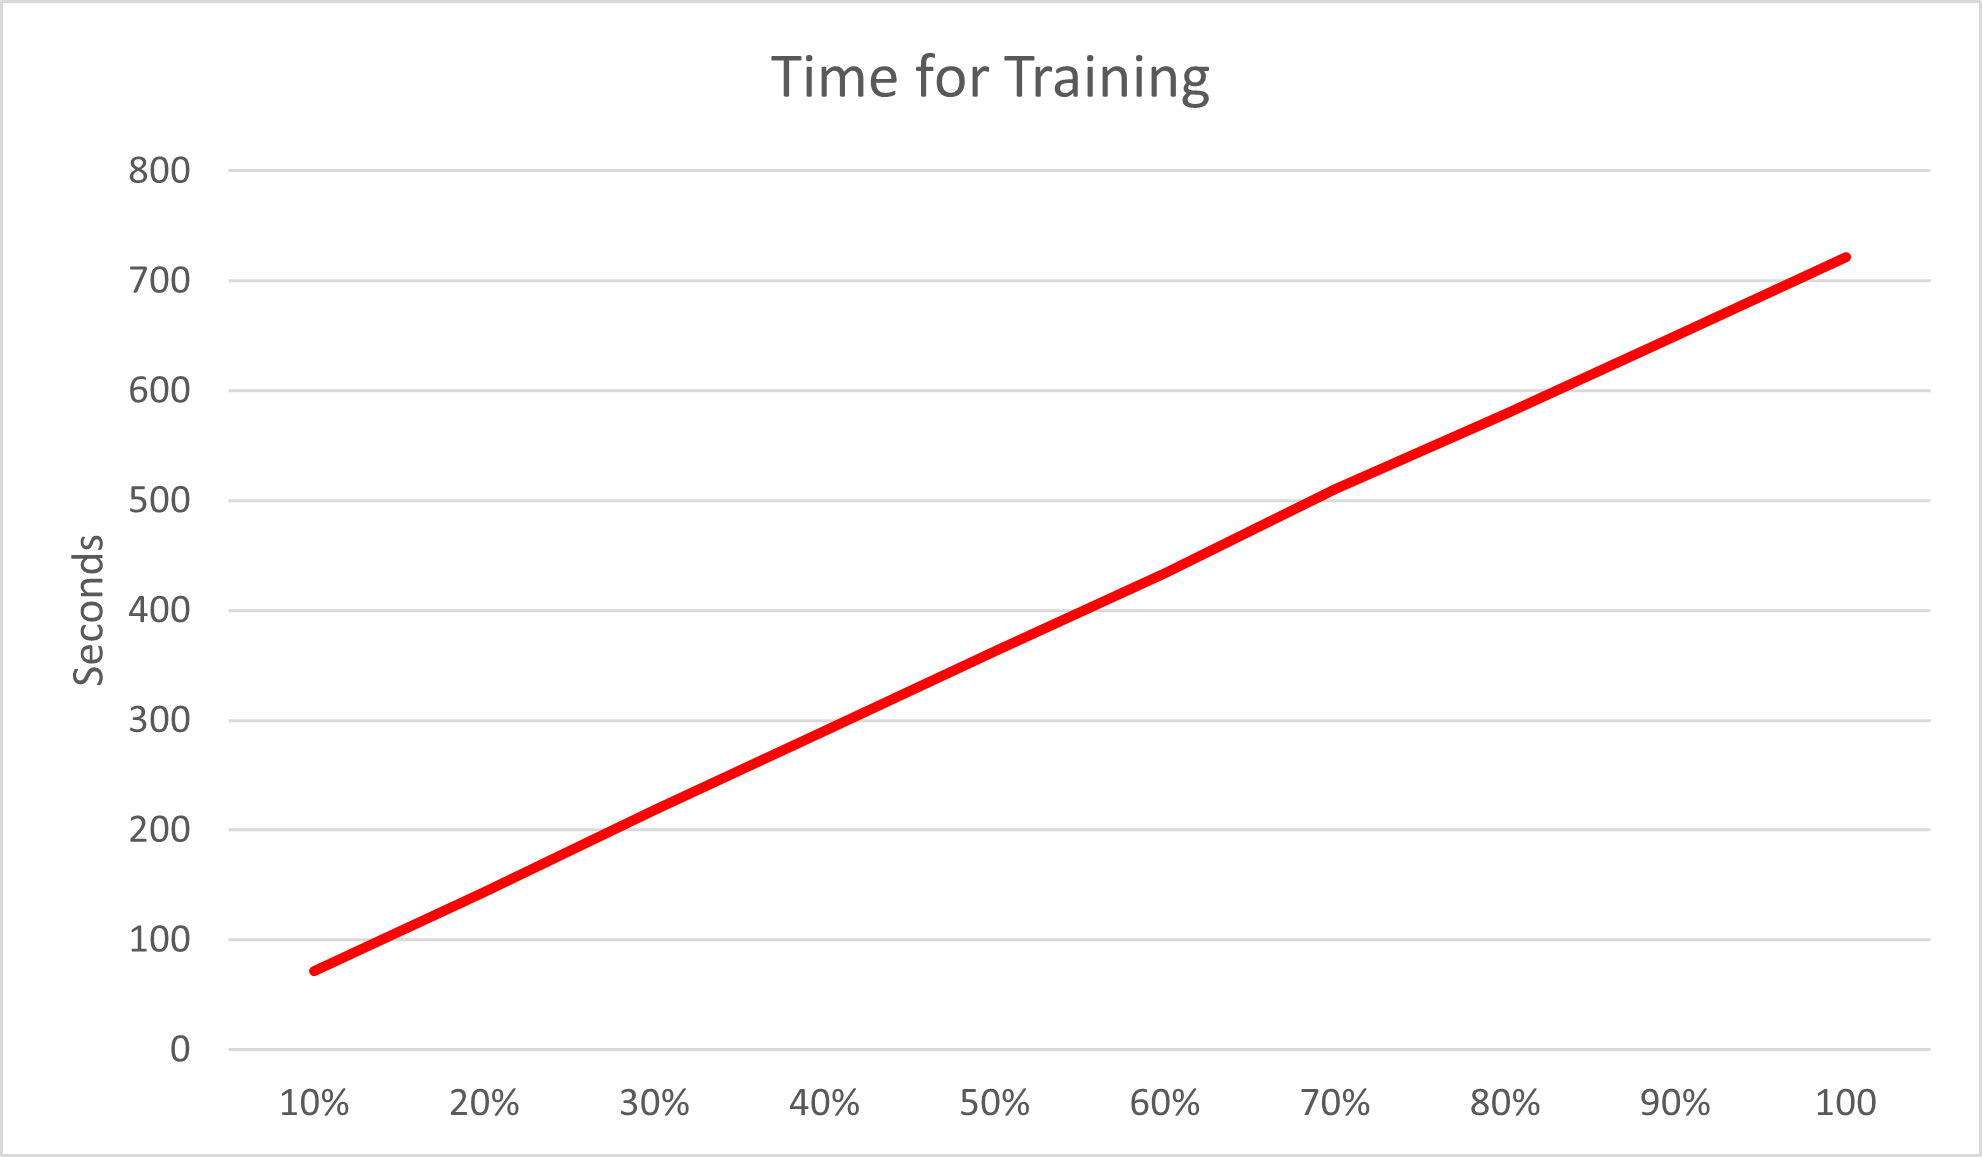
\includegraphics[width=0.7\textwidth]{Time for training KNN Digit.png}}
            \item 
            \caption{K Nearest Neighbor Digits Classifier Training Time}
        \end{figure}
\item
\begin{figure}[h!]
            \centering
            \IfFileExists{Accuracy KNN Digit.png}{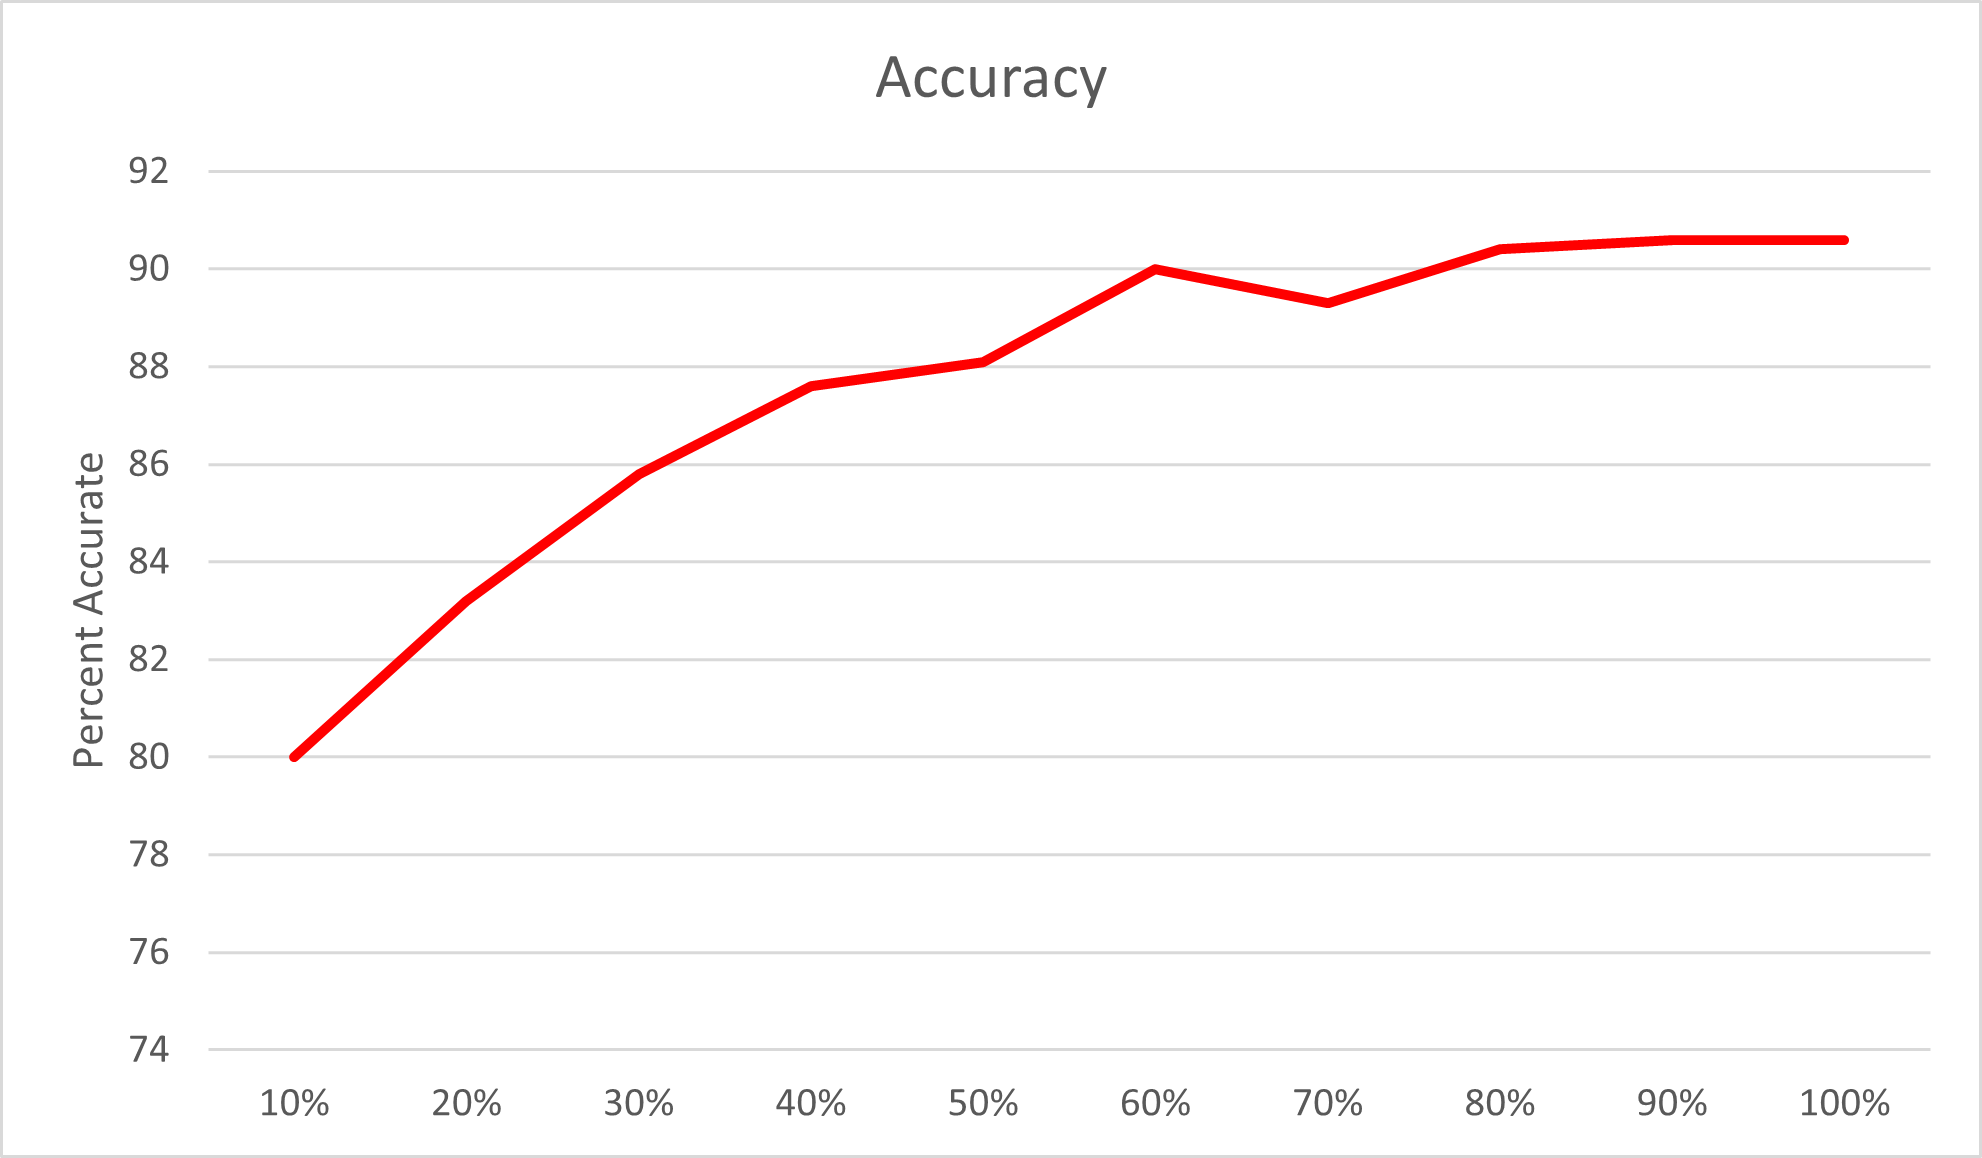
\includegraphics[width=0.7\textwidth]{Accuracy KNN Digit.png}}
            \item 
            \caption{K Nearest Neighbor Accuracy of Digits Classification}
        \end{figure}
        
\item
\begin{figure}[h!]
            \centering
            \IfFileExists{Standard deviation KNN Digit.png}{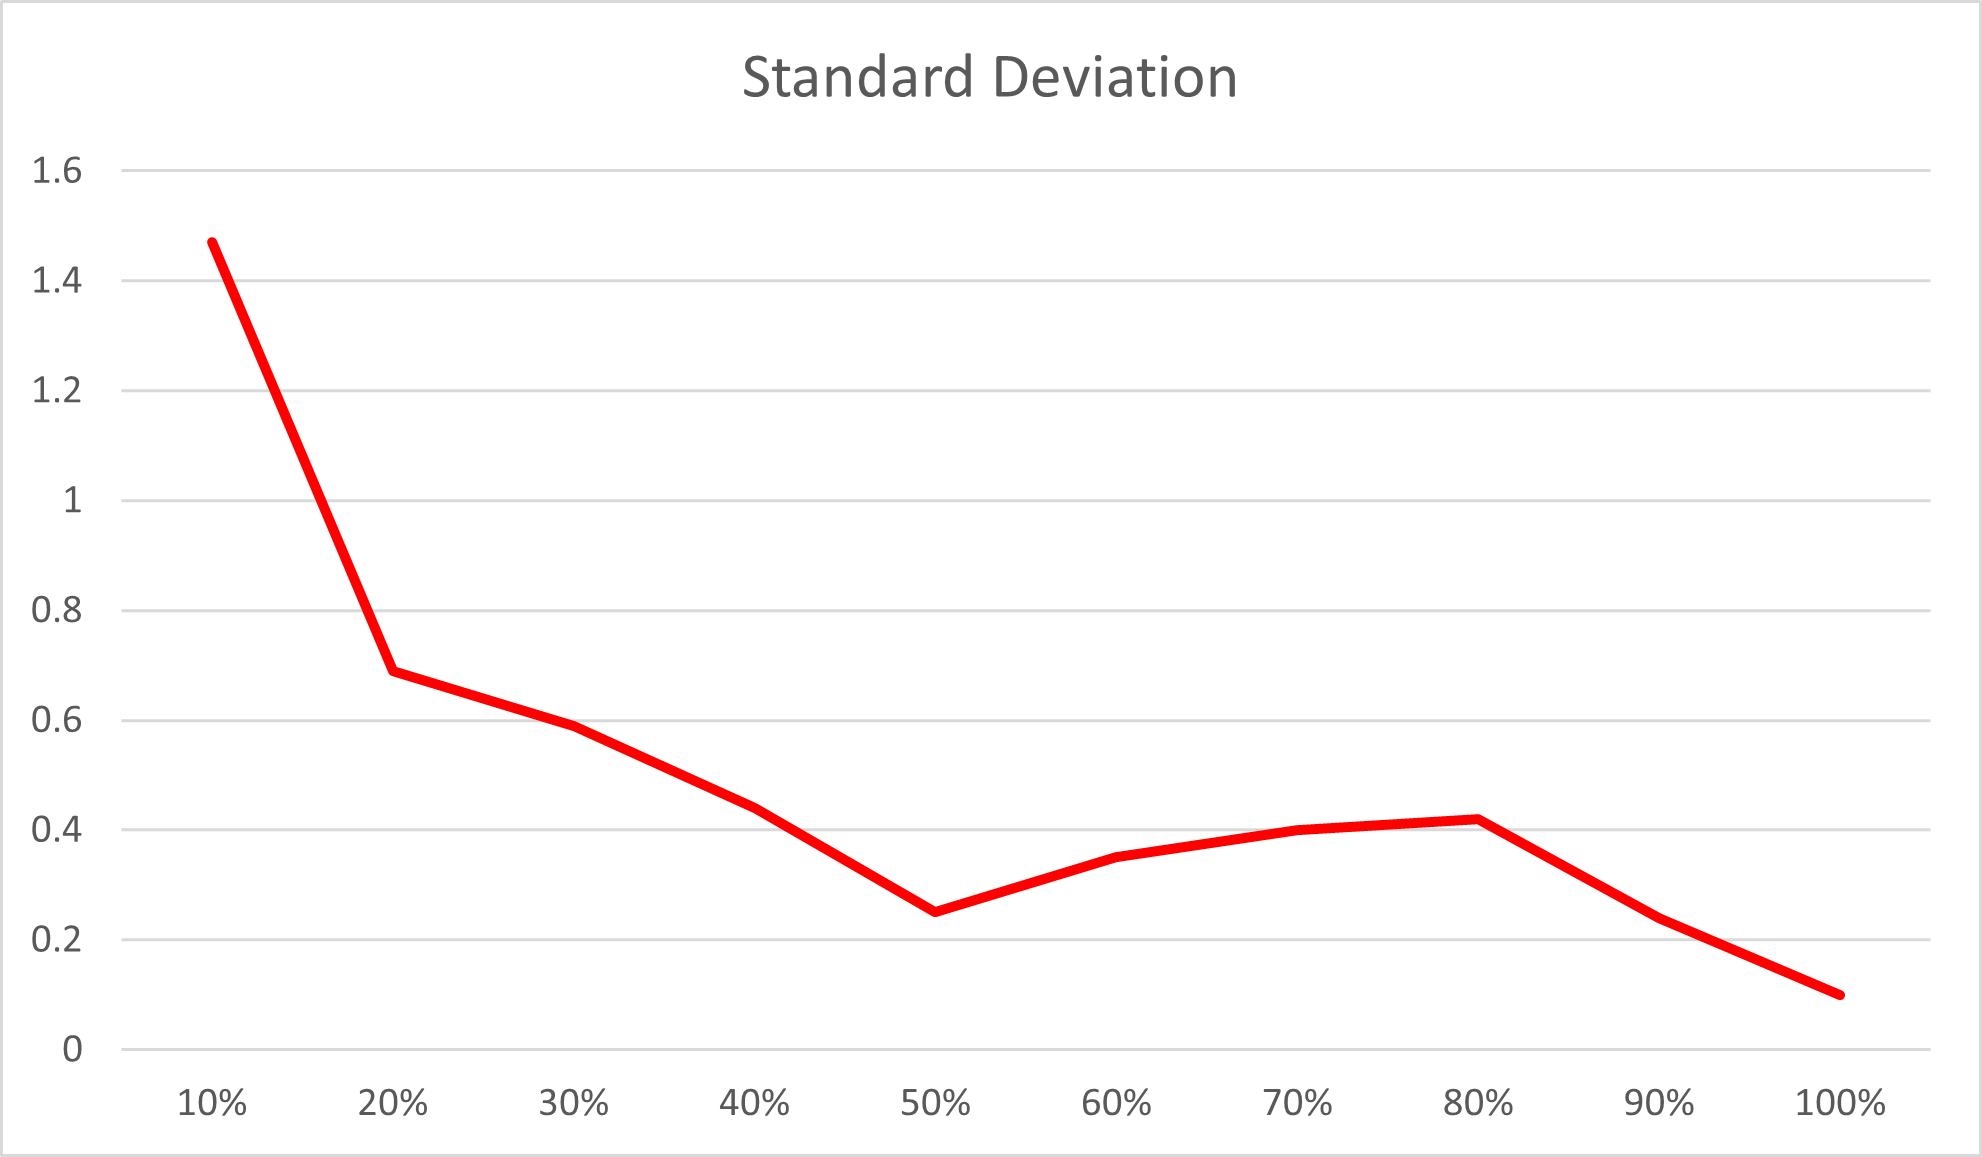
\includegraphics[width=0.7\textwidth]{Standard deviation KNN Digit.png}}
            \item 
            \caption{K Nearest Neighbor Standard Deviation of Digits Classification}
        \end{figure}

\begin{newpage}
\end{newpage}

\item \textbf{K Nearest Neighbor Classification of Faces}
\item For Faces classifying we tested our program in increments of 10\% (10\%, 20\%, 30\%,..., 90\%, 100\%), of the total training data size. Standard deviation and accuracy was found on 100\% of the total testing data size. The following graphs were created to show the time for training (in seconds), accuracy (in percentage), and standard deviation of the data sizes tested.

\begin{figure}[h!]
            \centering
            \IfFileExists{Time for training KNN Faces.png}{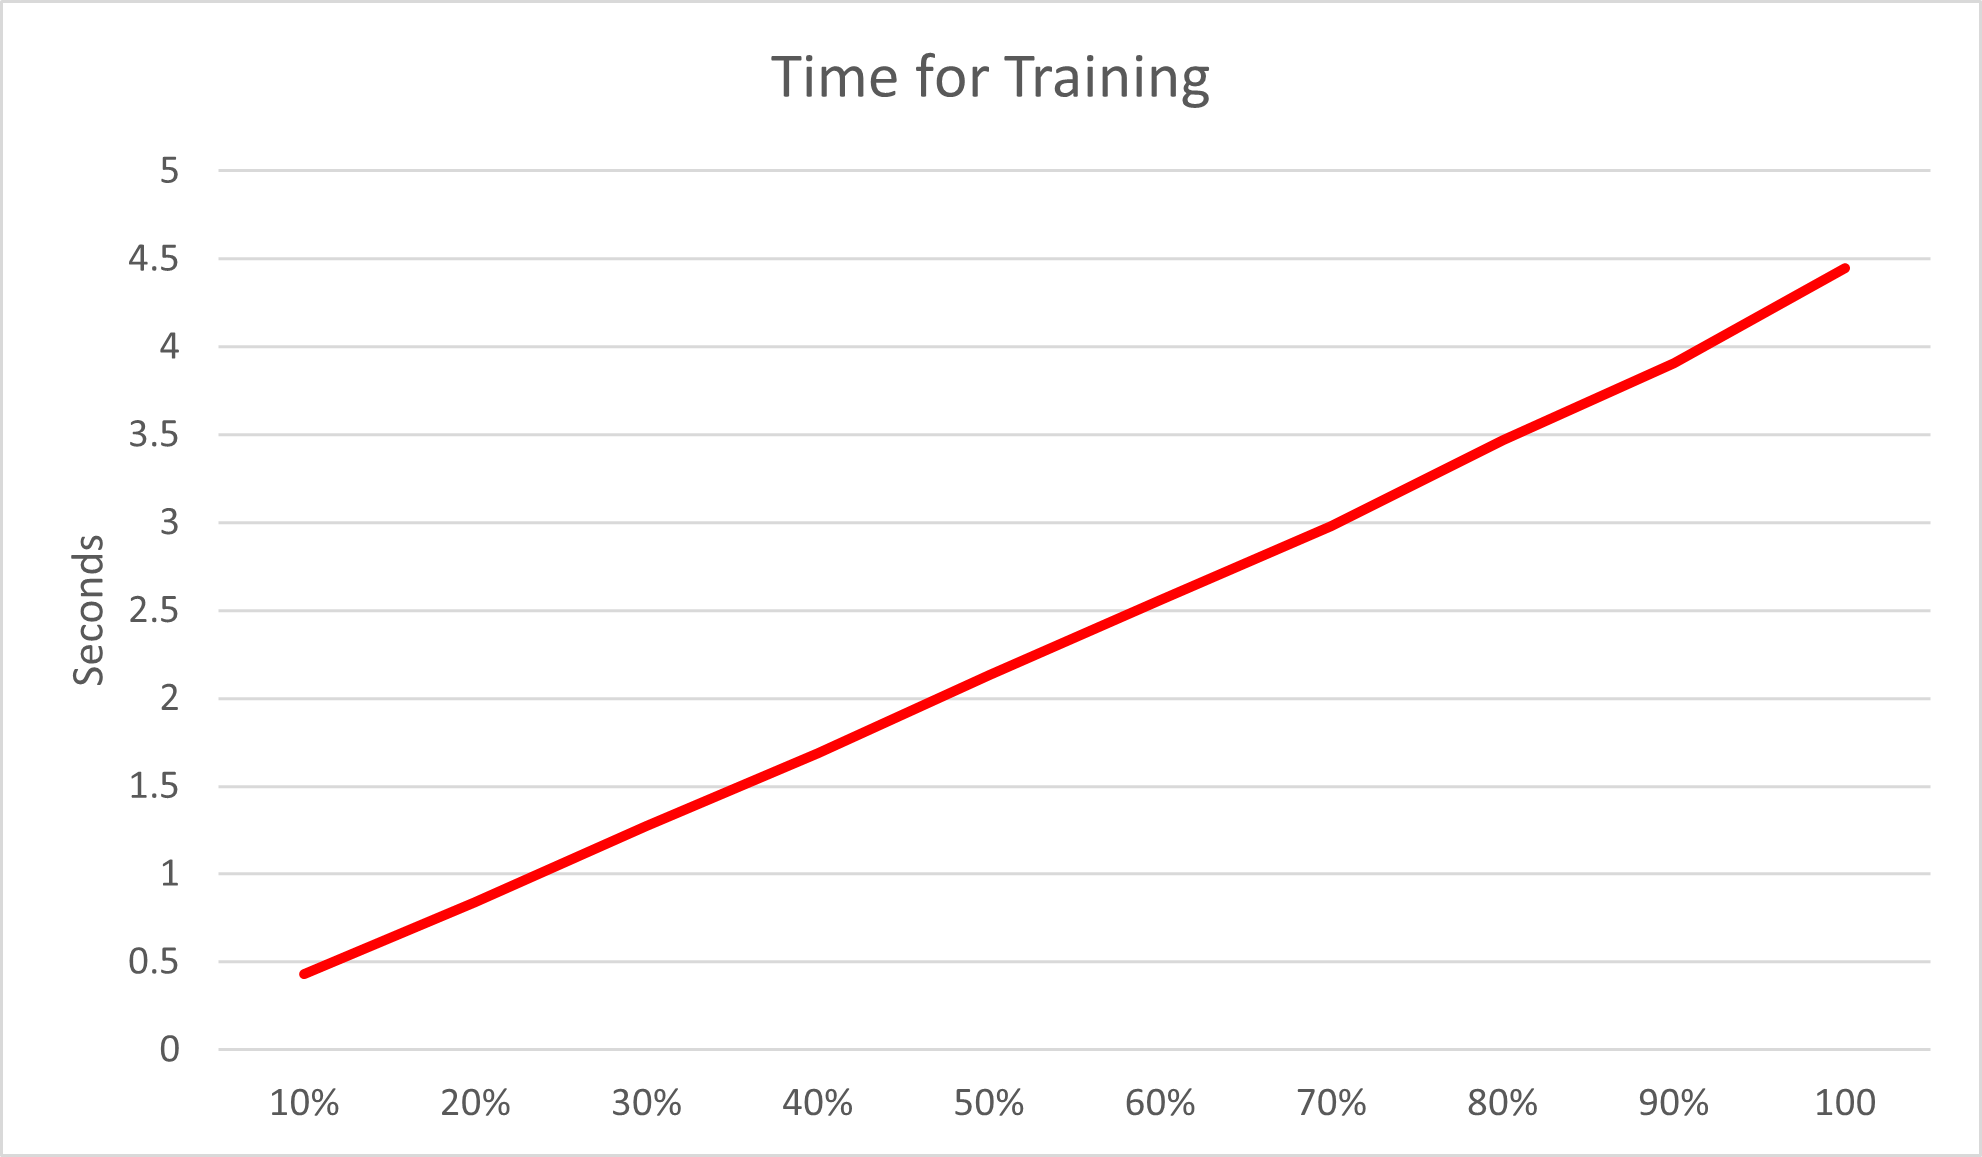
\includegraphics[width=0.7\textwidth]{Time for training KNN Faces.png}}
            \item 
            \caption{K Nearest Neighbor Faces Classifier Training Time}
        \end{figure}
\item
\begin{figure}[h!]
            \centering
            \IfFileExists{Accuracy KNN Faces.png}{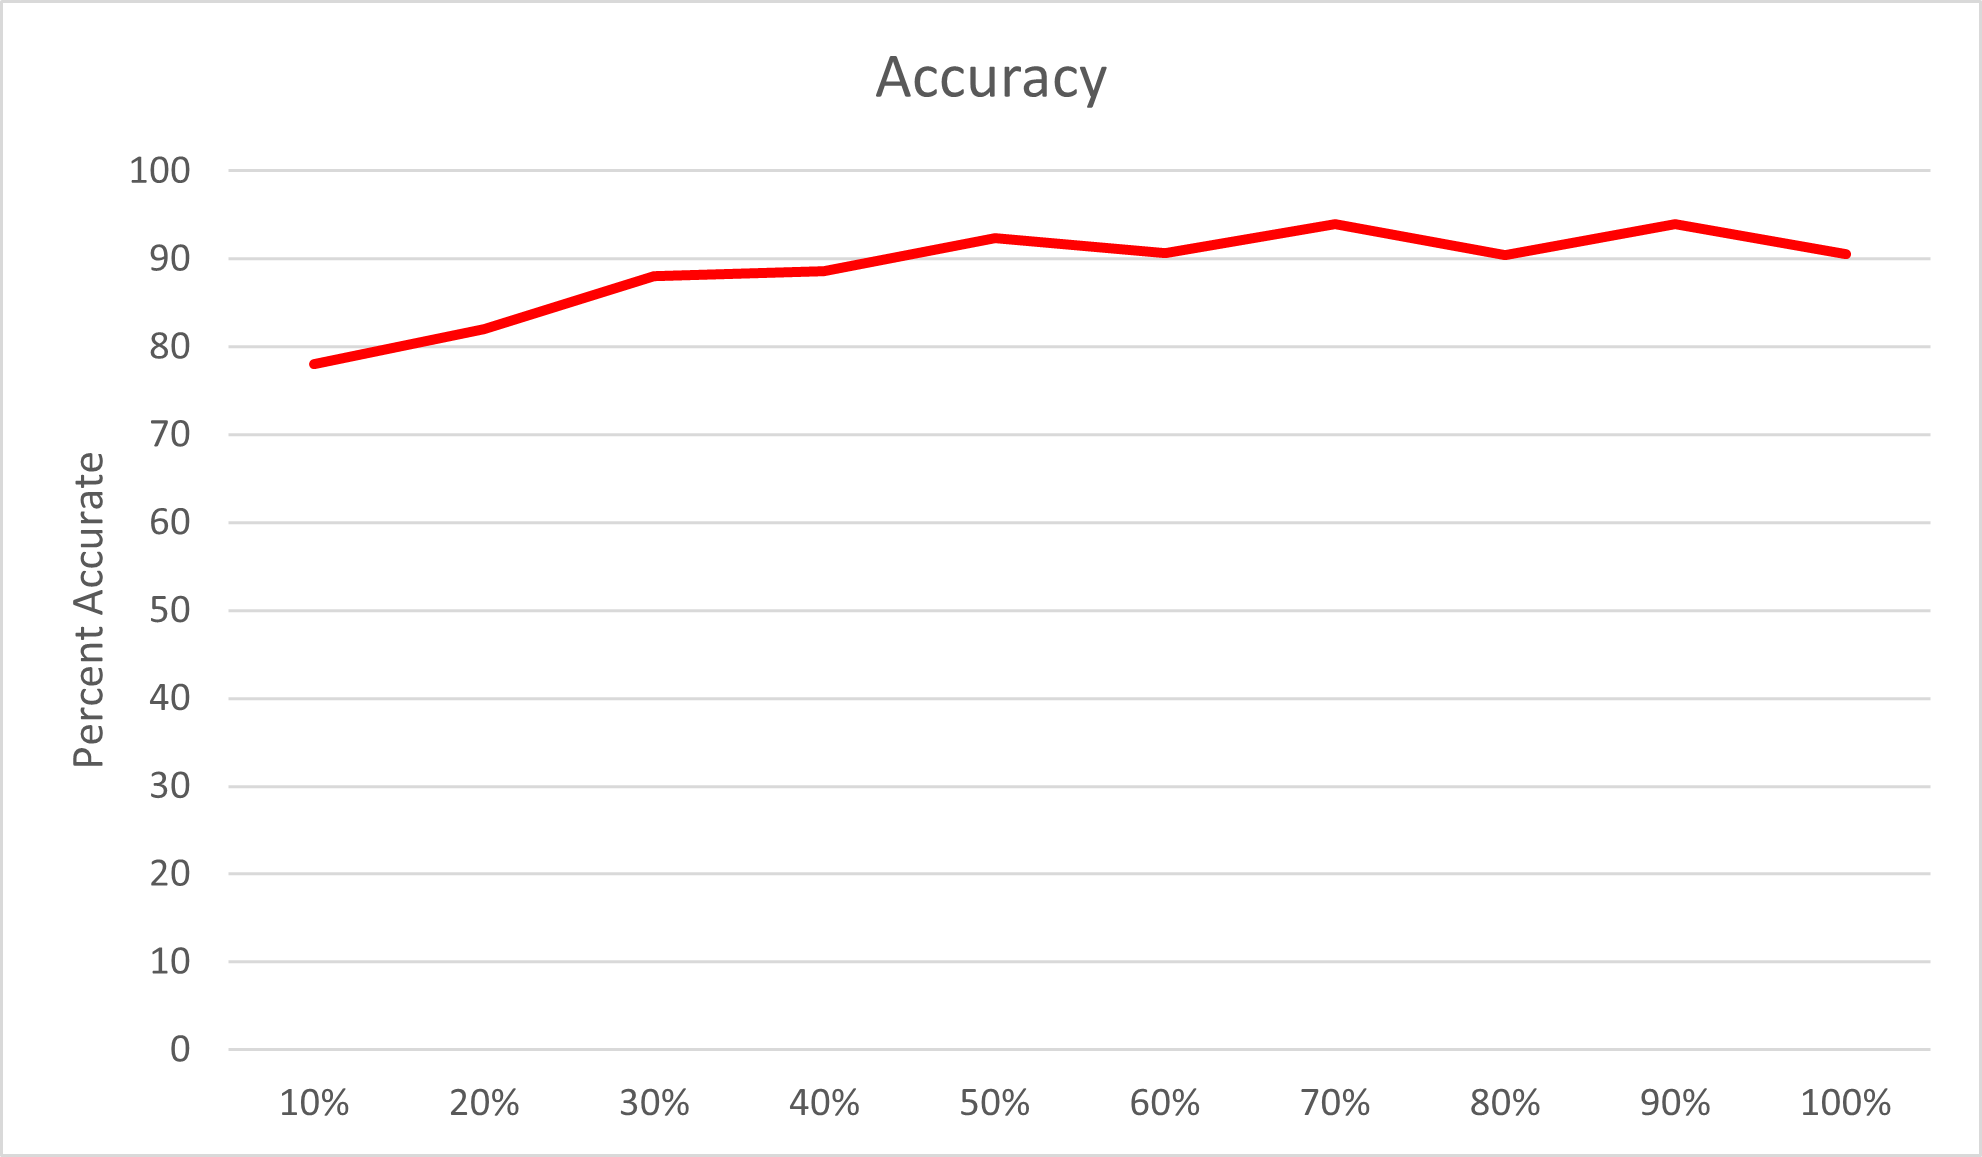
\includegraphics[width=0.7\textwidth]{Accuracy KNN Faces.png}}
            \item 
            \caption{K Nearest Neighbor Accuracy of Faces Classification}
        \end{figure}
        
\item
\begin{figure}[h!]
            \centering
            \IfFileExists{Standard deviation KNN Faces.png}{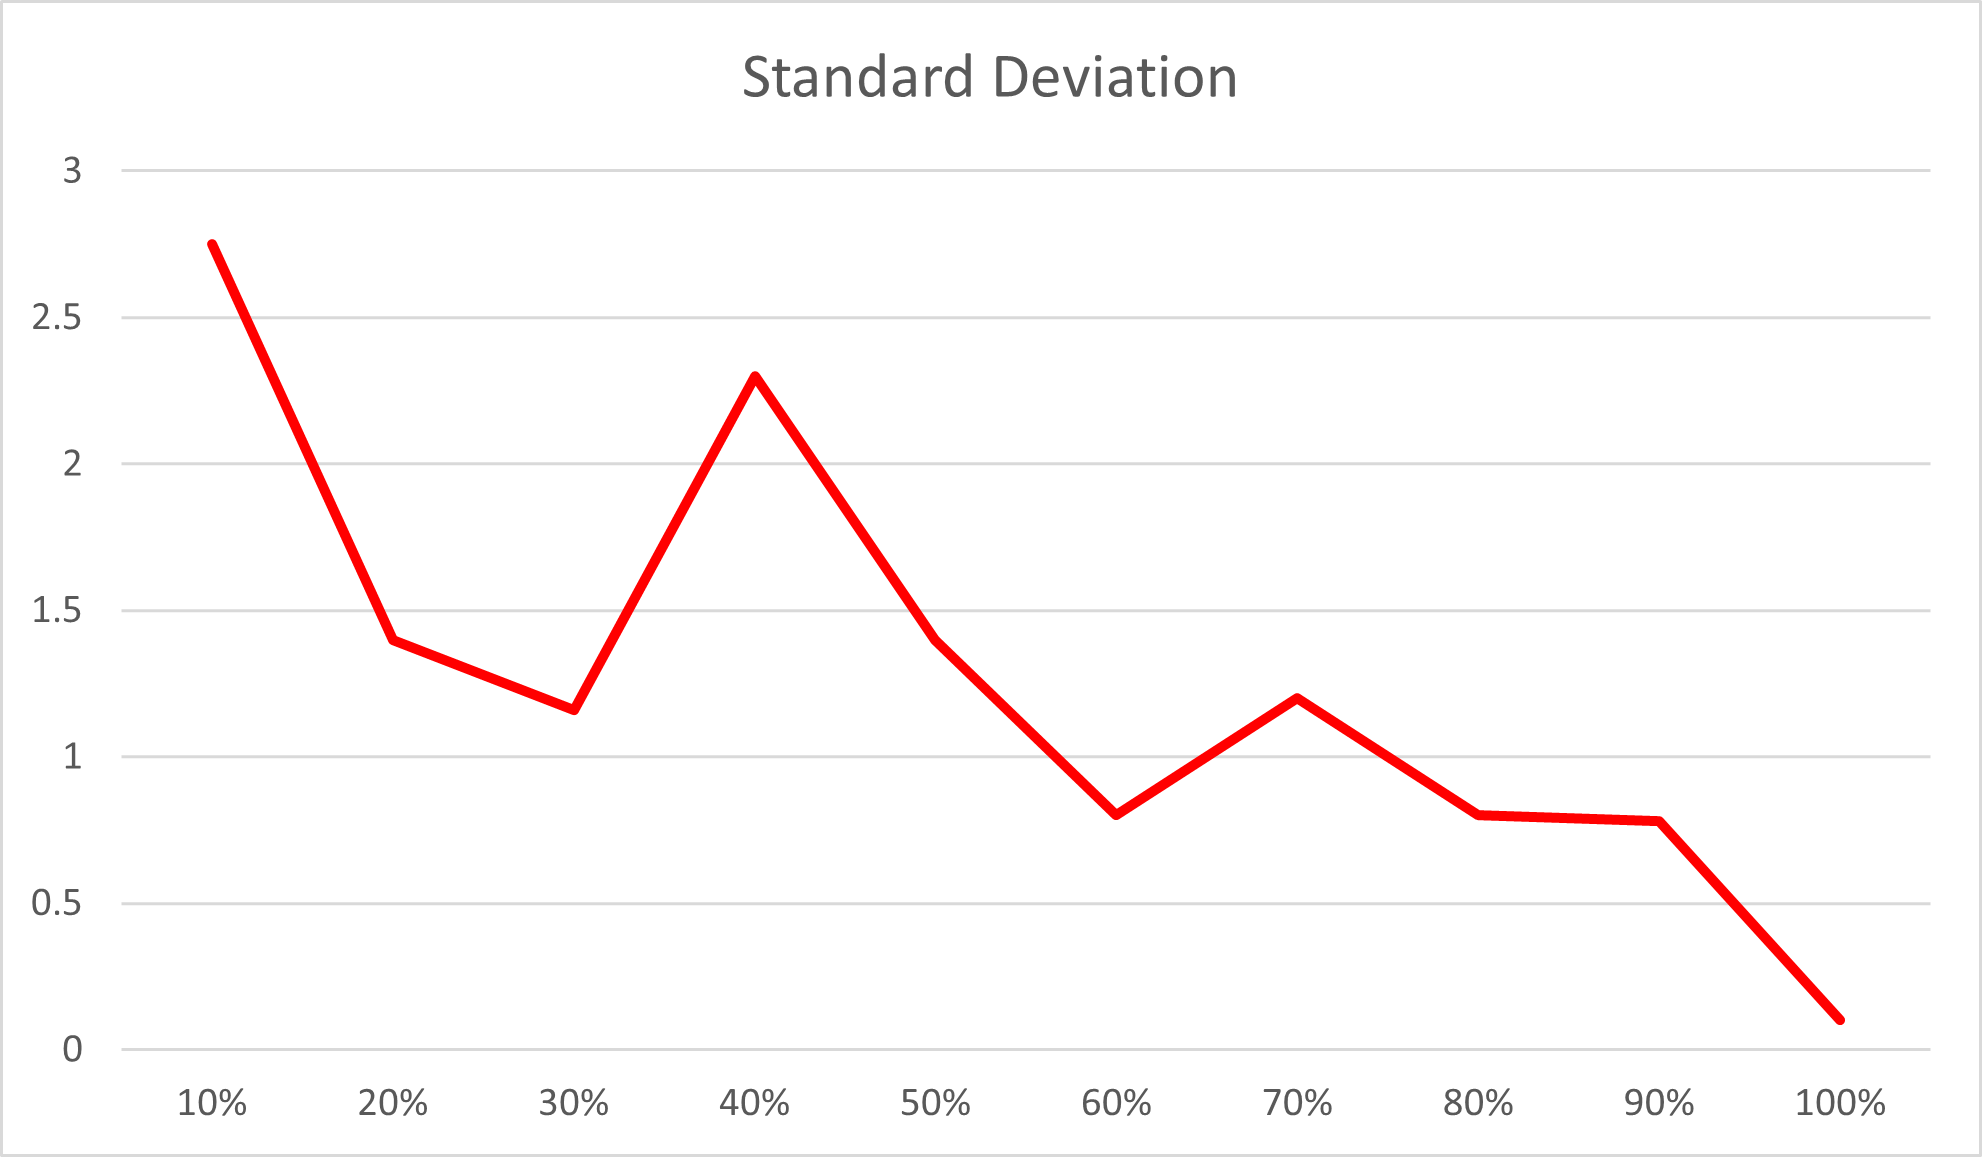
\includegraphics[width=0.7\textwidth]{Standard deviation KNN Faces.png}}
            \item 
            \caption{K Nearest Neighbor Standard Deviation of Faces Classification}
        \end{figure}

\begin{newpage}
\end{newpage}


\end{solution}

%---------------- PART 3 -----------------%
\begin{solution} \textbf{Part 3 - Discussion}

\item For all experiments performed, we crossed the 70\% accuracy barrier/goal for this project, given enough training. Time spent on the training process showed it was proportional to the amount of data provided. The more date provided, the longer it took to finish the training process. The opposite is also true (less time for less data).
\item For the accuracy of the programs, it was also proportional to the amount of data provided. This was mostly true for the beginning though. When the training data reached 40-50\%, it often maintained a certain accuracy level and did not drastically increase in performance after that point. Sometimes when the data is over fitting, the accuracy slightly decreased. 
\item For the standard deviation of the programs, it was proven to be inverse proportional for data provided in the beginning vs towards the end. Again, often around 40-50\% margin, the standard deviation did not drastically change after reaching that point as more data is provided. Sometimes the standard deviation increased when more data was provided and began over fitting. 

\end{solution}

%---------------- PART 4 -----------------%

\begin{solution} \textbf{Part 4 - Lessons We Learned}

\item The lessons we learned is that performance of an algorithm or program given more data does not guarantee more accuracy or better overall performance. The accuracy of the algorithms/programs would often settle near a certain point of accuracy, that point being dependent of the algorithm. When training a program, it is more efficient to perform an experiment or write an algorithm that finds which training data is optimal to finding that settling/converging point. That would better allow us to reduce run time of the training sequence and still meet the accuracy we expect.  

\end{solution}

%---------------- Resources Page -----------------%

\begin{newpage}
\end{newpage}
\begin{center}
\item \textbf{Resources}
\end{center}


\begin{center} Skeleton code and source files/project references \end{center}
\url{https://inst.eecs.berkeley.edu//~cs188/sp11/projects/classification/classification.html}
\begin{center} Laplace smoothing \end{center}
\url{https://towardsdatascience.com/laplace-smoothing-in-na\%C3\%AFve-bayes-algorithm-9c237a8bdece}
\begin{center} Perceptron youtube video
\item
\url{https://youtu.be/-KLnurhX-Pg}
\end{center} 


\end{document}